%!TEX root = thesis.tex

\chapter{Combining topics and domain expertise to develop insight into plankton ecology} \label{ch:plankton}

As we have seen, the spatio-temporal topic model is a powerful model for unsupervised classification of location specific data, and by carefully defining a feature function, we can achieve intuitive classifications that match human semantic annotations. However, our interpretation of the model's outputs has thus far been somewhat straightforward. In this chapter, we delve deeper into how topic models can be used for tasks beyond classification.

A key feature of the spatio-temporal topic model is that it excels at finding co-occurrences in data that can be explained by the region in which each observation occurred. In addition to leading to appealing maps, this property means that topic distributions are often easier to predict accurately than other non-smooth representations of a dataset. Further, given a predicted topic distribution and the topics themselves, the maximum likelihood feature distribution is trivial to produce.

In this chapter, we explore two approaches that take this approach to predict unobserved feature distributions. Our motivation is to develop methods that provide intuitive insight into scientific data. In these applications, it is important for models to act in concert with domain knowledge, and therefore, it is crucial that insights be in terms of observable data, rather than abstract topic representations. As we will show, by predicting the data through the spatio-temporal topic model we enable representations that make intuitive trends in the data evident, and thus directly suggest questions for further study.

\section{Phytoplankton community model}
In addition to contributions to the machine learning literature, in the work presented in this chapter, we aim to contribute to domain research in phytoplankton ecology. Phytoplankton are microscopic organisms that form the base of marine food webs. They produce chlorophyll and other pigments to harvest sunlight and fuel photosynthesis, so they can utilize $\mathrm{CO}_2$ and other nutrients to produce $\mathrm{O}_2$ and new organic matter. As such, they play critical roles in global biogeochemical cycles and in structuring marine ecosystems.  
Marine scientists have long used techniques to measure the amount of chlorophyll in a water sample as a proxy for phytoplankton biomass \citep{Lorenzen1966}. These methods are coarse and give only bulk indices, with no information about which species of phytoplankton are present. Phytoplankton are extremely diverse, however, and their community structure plays a major role in shaping ecosystems and their functions. As an extreme example, particular species are known to cause toxic blooms that can threaten wildlife as well as human health.

\begin{figure}
\begin{center}

\subfloat[]{
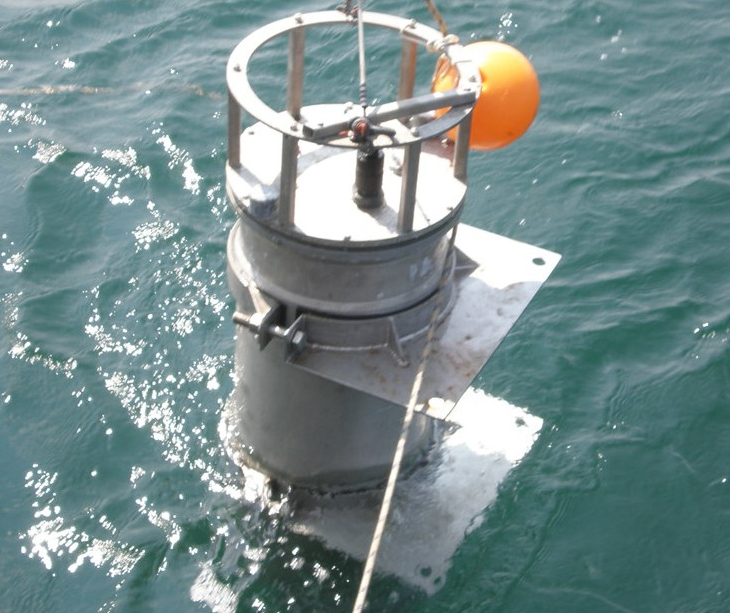
\includegraphics[width=0.45\columnwidth]{figures/oceans/IFCB.jpg}
\label{fig:ifcb-device}
}%
\subfloat[]{
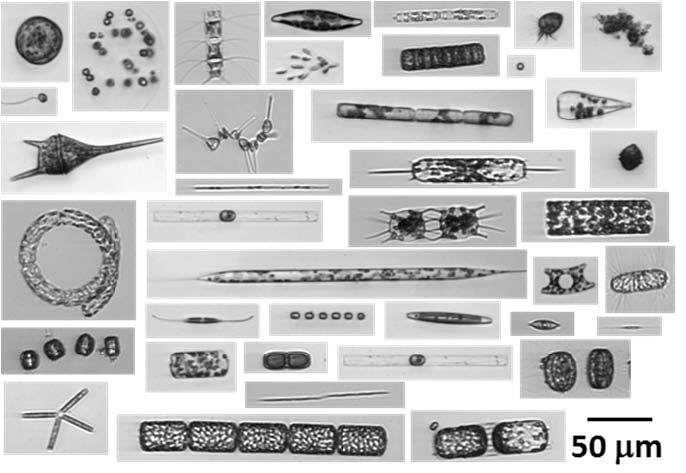
\includegraphics[width=0.54\columnwidth]{figures/icra_plankton/IFCB_collage.jpg}
\label{fig:ifcb-collage}
}
\end{center}
\caption{
\protect\subref{fig:ifcb-device} Imaging FlowCyto Bot (IFCB) being deployed at Martha's Vineyard, MA.
\protect\subref{fig:ifcb-collage} Example phytoplankton detections from IFCB.
}
\label{fig:ifcb}
\end{figure}

To meet the gap in observational capability that includes taxonomic resolution, Sosik and Olson have developed the automated, submersible Imaging FlowCytobot (IFCB, Fig.~\ref{fig:ifcb-device})~\citep{Olson2007a}. IFCB acts as an autonomous underwater microscope, collecting water samples and imaging small droplets at high resolution ($\sim$\SI{1}{\micro\meter}). The coupled analysis system \citep{Sosik2007} is able to detect and crop phytoplankton within these images (See Fig.~\ref{fig:ifcb-collage}). Many of these contain sufficient detail to be automatically classified to the genus or species level by a random-forest based system \citep{Sosik2016}. IFCB is designed to serially sample ocean water and perform detection and classification for long periods of time (weeks to years) with minimal manual intervention.

Sosik, Olson, and other IFCB users have collected impressively detailed datasets of plankton taxon (i.e. species or genus) abundance, both with long-term fixed location IFCB deployments, and over large areas by deploying IFCB underway on a ship.\footnote{Datasets available online at \url{http://ifcb-data.whoi.edu/mvco/}}
Nevertheless, this level of detail comes at the price of intuitive, comprehensive models using classic statistical techniques. To our knowledge, no other work has attempted to derive understanding about the interactions between multiple taxa in this dataset, nonetheless all of them considered together.

We hypothesize that by taking sparsity and spatio-temporal smoothness into account, a spatio-temporal topic model will be able to produce such an account without sacrificing interpretability. Specifically, the topic model's discrete-valued feature function is taken to be the occurrence of each taxon, and neighborhoods are taken to be the temporal or spatio-temporal windows in which the observations were made by IFCB. We interpret the resulting word-topic distributions as \emph{communities} -- probabilistic groupings of plankton taxa that tend to co-occur. Under this interpretation, the topic-neighborhood distributions describe the mixture of communities found in a given location.

Similar to previous examples in this thesis, we expect that each community should be mainly comprised of only a few taxa, that for any location few communities should be present, and that within some neighborhood the distribution of communities should be similar. By applying priors which prefer models that respect these conditions, we ensure that our community model will be not only accurate, but also easy to interpret.

As we have seen, the (spatio-) temporal topic model can be used to estimate the posterior probability of topic assignments $P(\boldsymbol{z} | \boldsymbol{w})$ via the collapsed Gibbs sampler update (in Eqn.~\ref{eqn:posterior}), and further that given a set of topic assignments, the posterior distributions for $\Theta$ and $\Phi$ are given by $Dir(\alpha + \boldsymbol{N}_{g(x)}^{1:K})$ and $Dir(\beta + \boldsymbol{N}_k^{1:V})$ respectively. The mean of a Dirichlet distribution is its parameter normalized, so the maximum likelihood estimate (MLE), denoted $\hat{\Theta}$ and $\hat{\Phi}$ are trivial to recover

\begin{equation} \label{eqn:mle_thetaphi}
\hat{\Theta}_{g(x), k} = \frac{N^k_{g(x)} + \alpha}{\sum_{j=1}^K N^j_{g(x)} + \alpha}, \quad
\hat{\Phi}_{k,w_i} = \frac{N^{w_i}_k + \beta}{\sum_{v=1}^V N^v_k + \beta},
\end{equation}

To tie our communities back to the domain of phytoplankton observations, we consider learning the community model, but also additional means of estimating the MLE community distributions when the phytoplankton observations themselves are not available. Supposing we have some method to estimate of these community distributions $\check{\theta} \approx \hat{\theta}$, we can in turn estimate the distribution of phytoplankton taxa
\begin{equation} \label{eqn:word-estimate}
P(w = v | \theta, \Phi) = \sum_{k=0}^K \theta_k \Phi_{k,v} \approx \sum_{k=0}^K \check{\theta}_k \hat{\Phi}_{k,v}
\end{equation}

A final issue in the formulation of our phytoplankton community model is that because these datasets are so unique, to our knowledge no domain research has attempted to define phytoplankton communities, and therefore we do not have strong information about how to set the number of topics $K$. For this reason, instead of fixing $K$ ahead of time, we apply a Dirichlet process (DP) prior on $\theta$ and learn the number of topics from data following the Bayesian non-parametric approach of \citep{Girdhar2016}, (BNP-ROST).

The DP is an infinite-dimensional generalization of the Dirchlet distribution, often used as a prior for infinite mixture models, where the number of components is not known \emph{a priori}. It is parameterized by a probability distribution $G$ with support set $A$, and a positive, real-valued scale parameter $\eta$. It is defined by the property that any finite partition of $A$ (a disjoint, covering set of subsets) is jointly Dirichlet distributed, i.e. for all finite partitions $\{A_0, \ldots, A_r\}$ \citep{Teh2010}
\begin{equation}
H \sim DP(\eta, G) \Rightarrow (H(A_0), \ldots, H(A_r)) \sim Dir(\eta G(A_0),\ldots,\eta G(A_r))
\end{equation}
In the Bayesian non-parametric topic model, a DP prior is placed on $\theta$. $A$ is considered to be the set of possible topic assignments for a word, with no limit on the maximum possible value. The key insight is that for any number of topics currently in use, $K$, the distribution over the partition with an element for each of the $K$ topics, plus another for any other possible topic assignment, i.e. the partition $\{z = 0, z = 1, \ldots, z = K - 1, z \geq K\}$, is a (finite) Dirichlet. We can view this in terms of the `Chinese Restaurant Process' construction, reparameterizing $G$ and $\eta$ in terms of our original symmetric Dirichlet parameter $\alpha$ and the probability $\gamma$ of incrementing the number of topics \citep{jordan2005}. This interpretation leads to a predictive distribution which is only a minor modification from the Dirichlet predictive distribution (Eqn.~\ref{eqn:posterior}):
\begin{equation}
\begin{aligned}
P(z_i = k | \boldsymbol{z_{-i}}) =
\begin{cases}
\frac{(N^k_{g(x)} + \alpha)}{\gamma + \sum_{j=1}^K N^j_{g(x)} + \alpha} & \mathrm{if}~k < K\\
\frac{\gamma}{\gamma + \sum_{j=1}^K N^j_{g(x)} + \alpha} & \mathrm{if}~k = K
\end{cases}
\end{aligned}
\end{equation}
where $K$ is incremented whenever some $z=K$ is drawn from the resulting distribution.

\section{Learning communities that are explained by the environment} \label{sec:plankton-seasonal}
Our first study involving IFCB plankton data aims at learning an interpretable community model for a fixed-location deployment at Martha's Vineyard Coastal Observatory (MVCO), one mile off the south-shore of Martha's Vineyard, MA \citep{Kalmbach2017}. In addition to an IFCB, MVCO has a suite of other sensors, enabling inquiry into the relationships between phytoplankton abundance and environment variables including oceanographic and meteorological factors such as dissolved $\mathrm{0}_2$ content, salinity, air and water temperature, and rainfall. While the combination of these two data sources could be used as the basis to learn intricate models of the precise relationship between each taxon and the environment, in this work we show that by first accounting for the associations between taxa, our method can capture most of the same information while requiring minimal domain knowledge.

We propose to use a simple simple linear-ridge regressor to predict the distribution of phytoplankton taxa from environment variables. We first train the community model and compute the MLE $\hat{\Theta}$ and $\hat{\Phi}$. Because of the prior imposed by our model, $\hat{\Theta}$ is relatively low-dimensional, sparse, and temporally smooth in comparison to the full phytoplankton distributions. Therefore, we hypothesize that estimating the communities and predicting the phytoplankton taxa by Eqn.~\ref{eqn:word-estimate} will produce more reliable predictions than a direct regression technique.

 In addition, this regression task provides complementary feedback to the topic model, ensuring that the final community model is both interpretable and accurate. For this application, instead of using the probability of held-out data as the cross-validation metric, we propose to use the agreement (which we define as $1/D_{KL}$) between the predicted taxon distributions based on environmental factors and the ground-truth taxon distribution. By doing so, we ensure that the maximum likelihood taxon distributions given the topics closely resemble the true taxon distributions, but also that the topic distributions themselves can be explained simply in terms of the chosen environment variables. For this reason, rather than choosing a complex regression model, which may have better overall performance on the final predictions, we take an unsophisticated linear ridge approach to regression.

\subsection{Martha's Vineyard multi-year timeseries experiment}
We demonstrate our method on a dataset recorded continuously from Jan. 2009 to Jul. 2016 at MVCO. IFCB was configured to automatically sample from 5 ml of surface seawater approximately every 20 min. The classification system generated an average of over 1100 observations per day, distributed over 47 taxa (Fig.~\ref{fig:plankton-mvco-gt}).

We aggregated the observations to produce the taxon distribution for each day during the 7.5 year period, and used this as input to our method. For the regression model, we chose a suite of 18 environment variables from the MVCO ocean data and meteorological data summaries (Fig.~\ref{fig:plankton-mvco-regression-inputs}). In addition to being naively chosen, the environment data features significant gaps and systematic noise due to the practical challenges of long-term ocean sensor deployments. Much of the systematic noise was suppressed by rejecting outliers based on the median absolute deviation of each variable, yet the regression task remains extremely challenging.

\begin{figure}
    \centering
    \begin{subfloat}
        \centering
        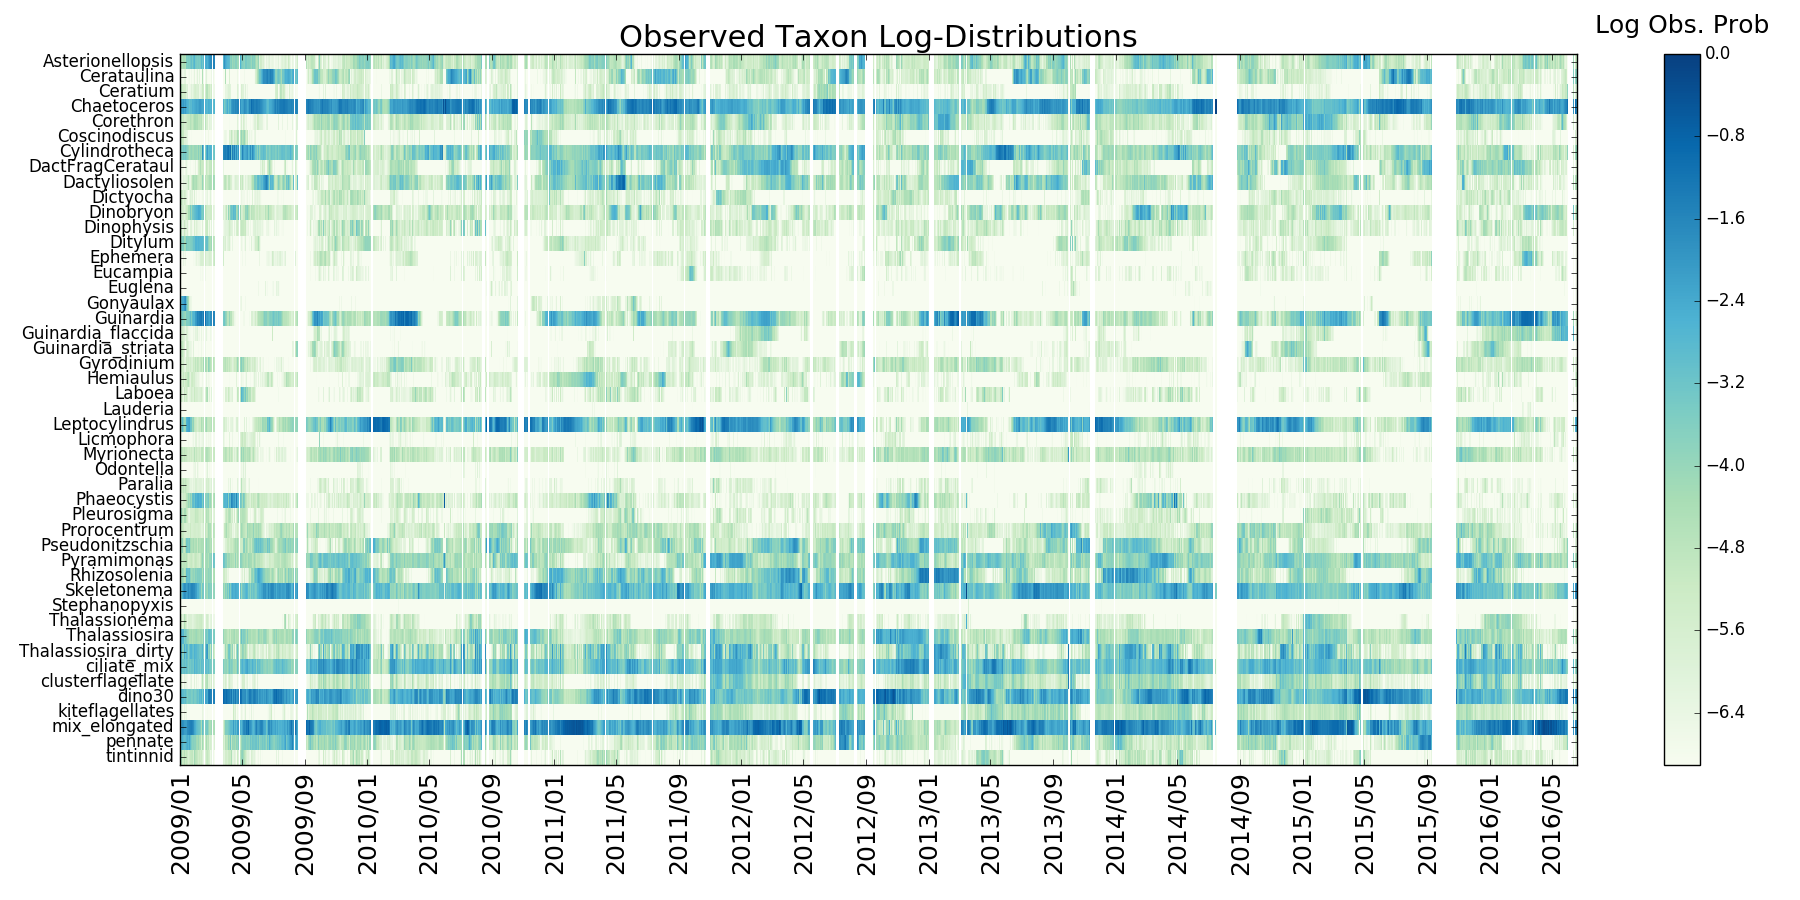
\includegraphics[width=0.85\textwidth]{figures/oceans/taxa_distros_gt.png}
        \caption{Observed daily taxon log-distributions at Martha's Vineyard Coastal Observatory over 7.5 years.}
        \label{fig:plankton-mvco-gt}
    \end{subfloat}
    \begin{subfloat}
        \centering
        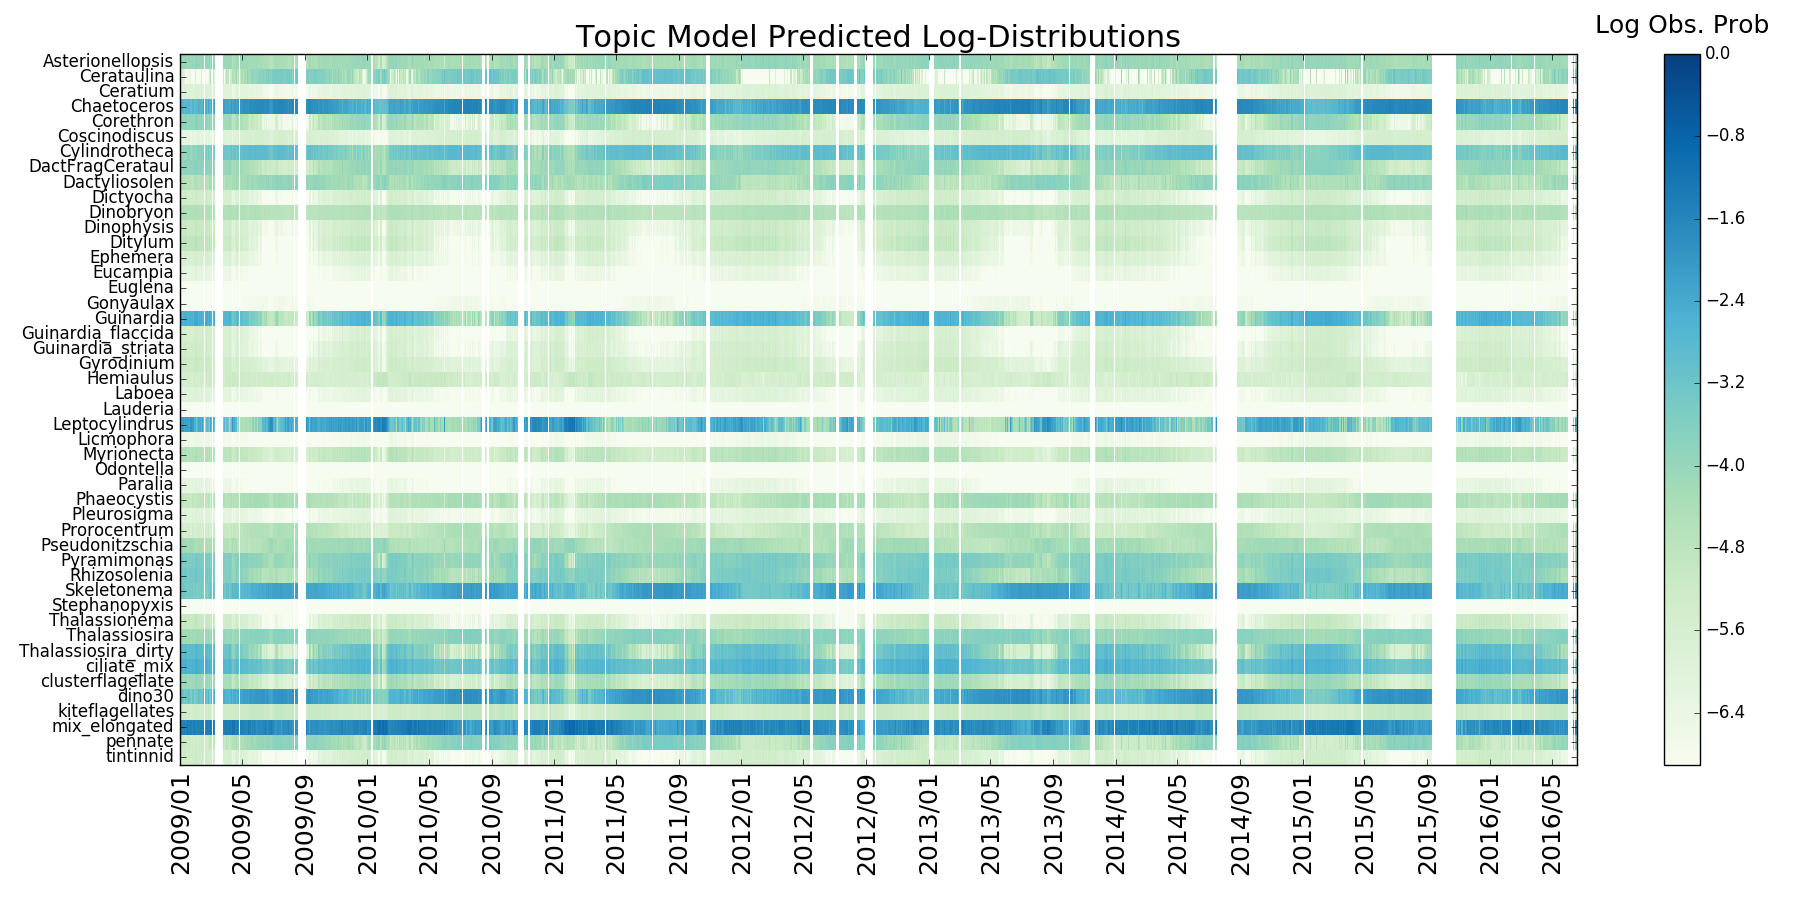
\includegraphics[width=0.85\textwidth]{figures/oceans/taxa_distros_hat_topics.png}
        \caption{Predicted taxon log-distributions using our community model and regression system.}
        \label{fig:plankton-mvco-topic-est}
    \end{subfloat}%
\end{figure}
\begin{figure}
	\ContinuedFloat
    \centering
    \begin{subfloat}
        \centering
        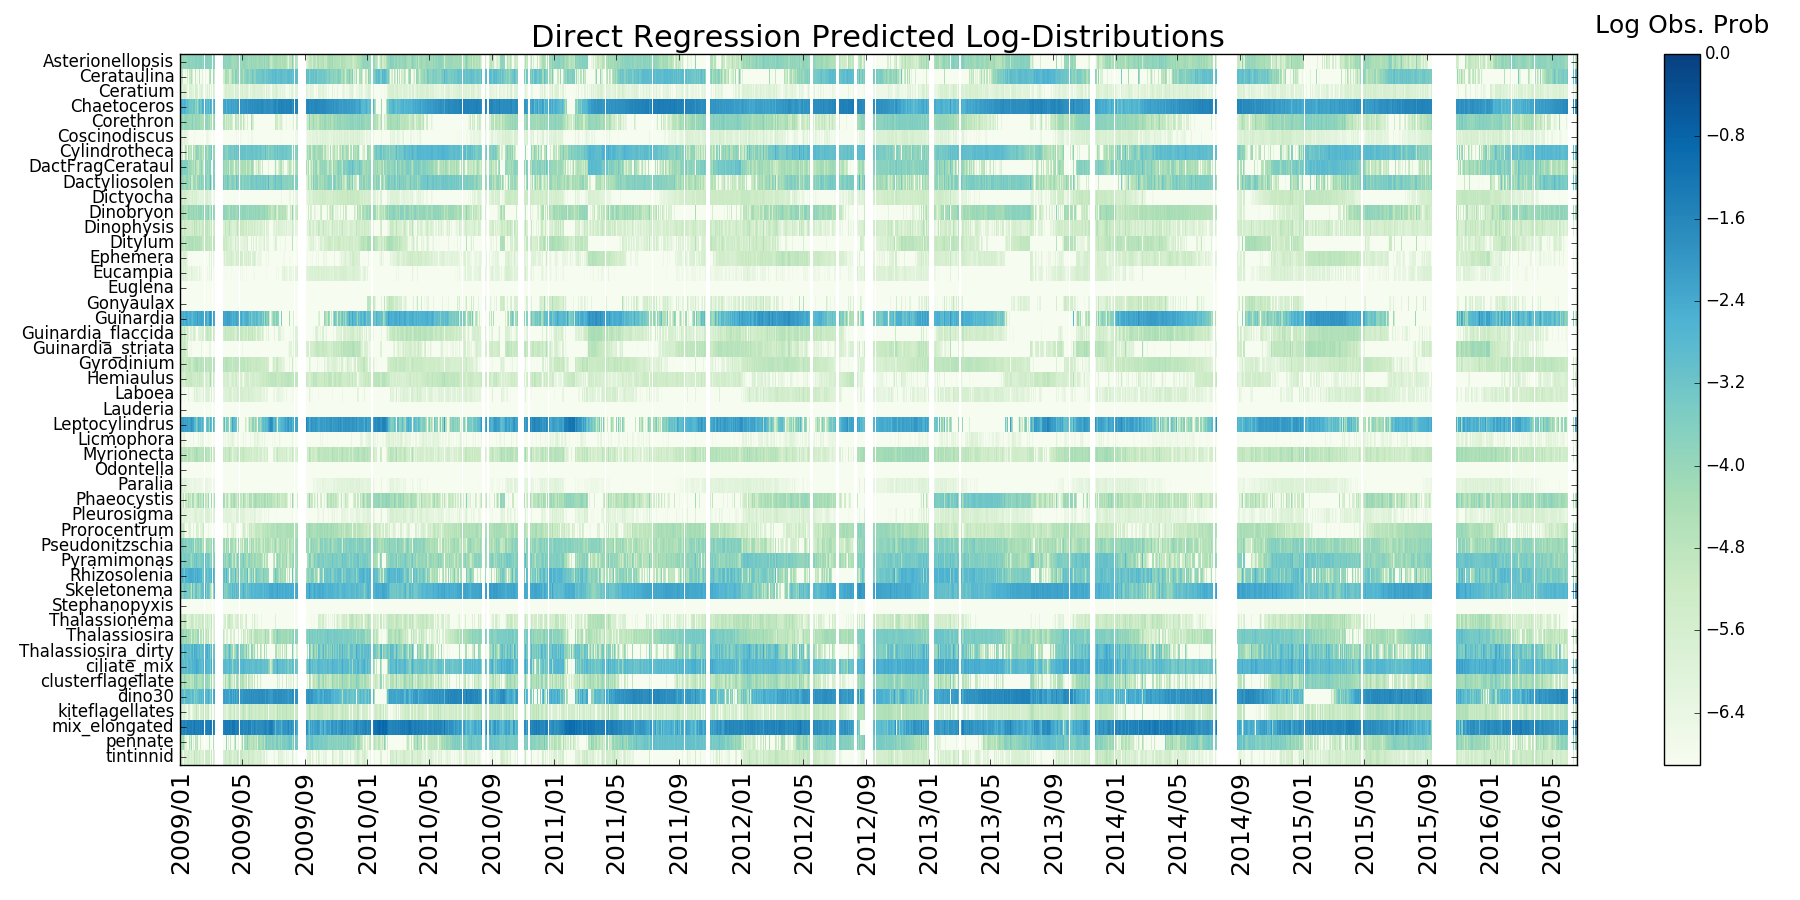
\includegraphics[width=0.85\textwidth]{figures/oceans/taxa_distros_hat_words.png}
        \caption{Predicted taxon log-distributions using direct regression on taxon distributions.}
        \label{fig:plankton-mvco-word-est}
    \end{subfloat}
    \caption{}
    \label{fig:plankton-mvco}
\end{figure}

\begin{figure}
    \centering
    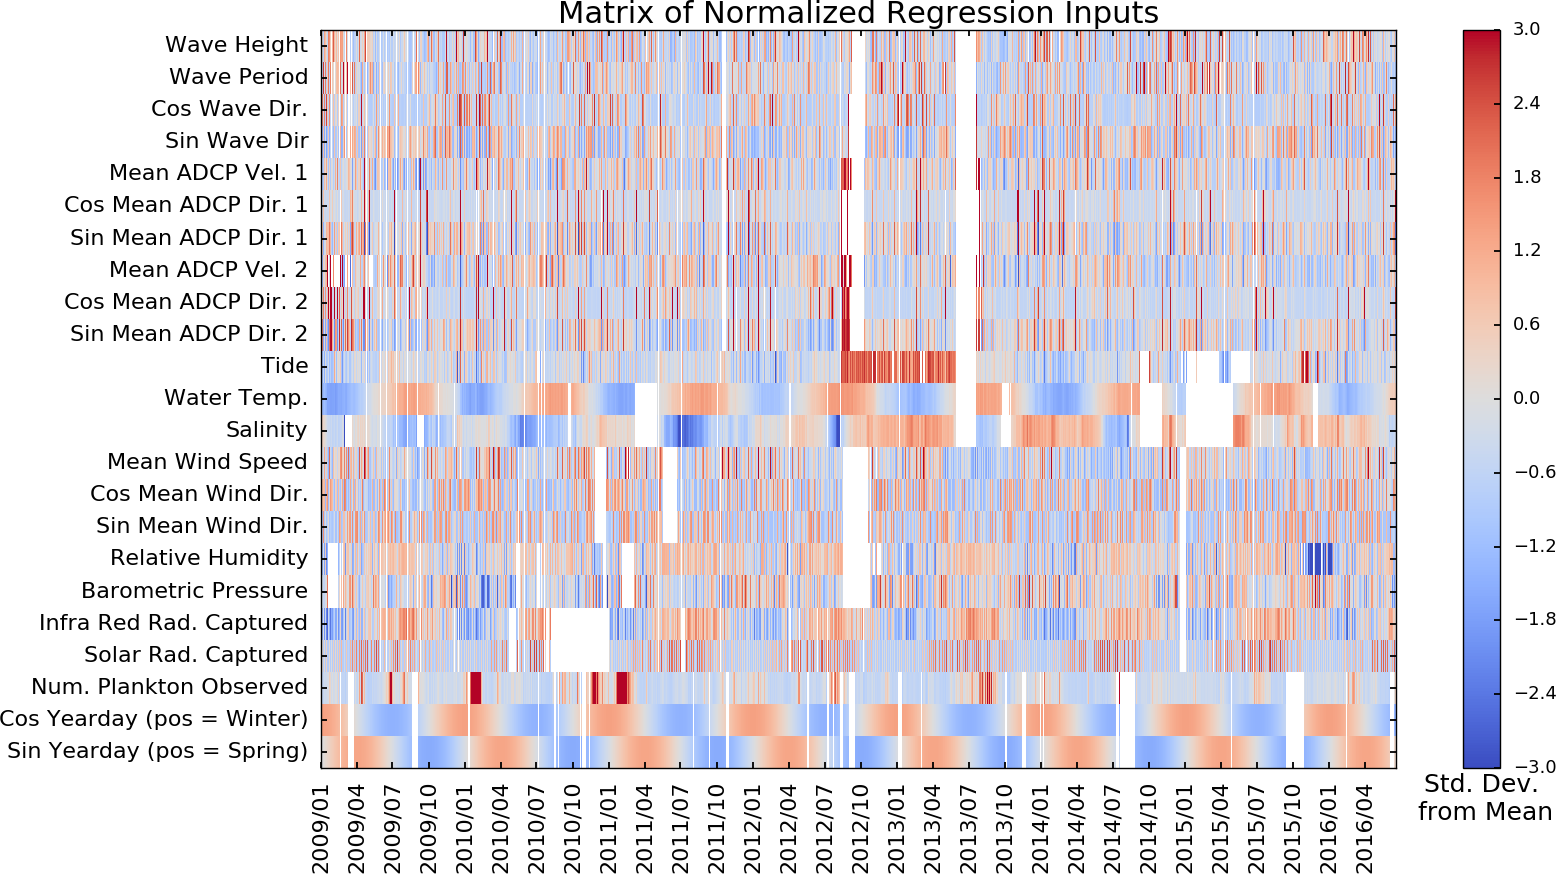
\includegraphics[width=0.9\textwidth]{figures/oceans/RegressionInputsNorm.png}
    \caption{\emph{Environment variables used to predict phytoplankton distributions}:
    Oceanographic and meteorological factors potentially related to phytoplankton life-cycles, centered and scaled to a normal distribution as our regression system receives them. White spaces indicate gaps in the data or where outlier data was removed.}
    \label{fig:plankton-mvco-regression-inputs}
\end{figure}

We trained our community model on the taxon distributions over the entire period multiple times for different hyperparameter settings, varying the topic concentration $\alpha$, the topic-prior concentration $\beta$, the DP prior parameter $\gamma$, and the neighborhood size $g$. For each community model corresponding to a different combination of choices of these hyperparameters, we trained the regression model 8 times, once using each year as the test set and the other 6.5 years for training. Within each training set, we chose the regularization parameter for ridge regression using hold-one-out cross validation. Finally, we used the resulting regressors to predict the respective held-out community distributions for each year, and used the respective community models to predict the taxon distributions.

We demonstrate the utility of our method in comparison to two more standard regression techniques. The first is to predict the taxon distributions directly with a similar ridge regression model and training procedure. The second is to first take a PCA decomposition of the taxon count data, using the first $K$ principle components, where $K$ is the same as the number of communities used by our model, and then use the same ridge regression model and training procedure to predict the PCA weights, and finally project the weights back to predict the taxon distributions.

\begin{figure}
    \centering
    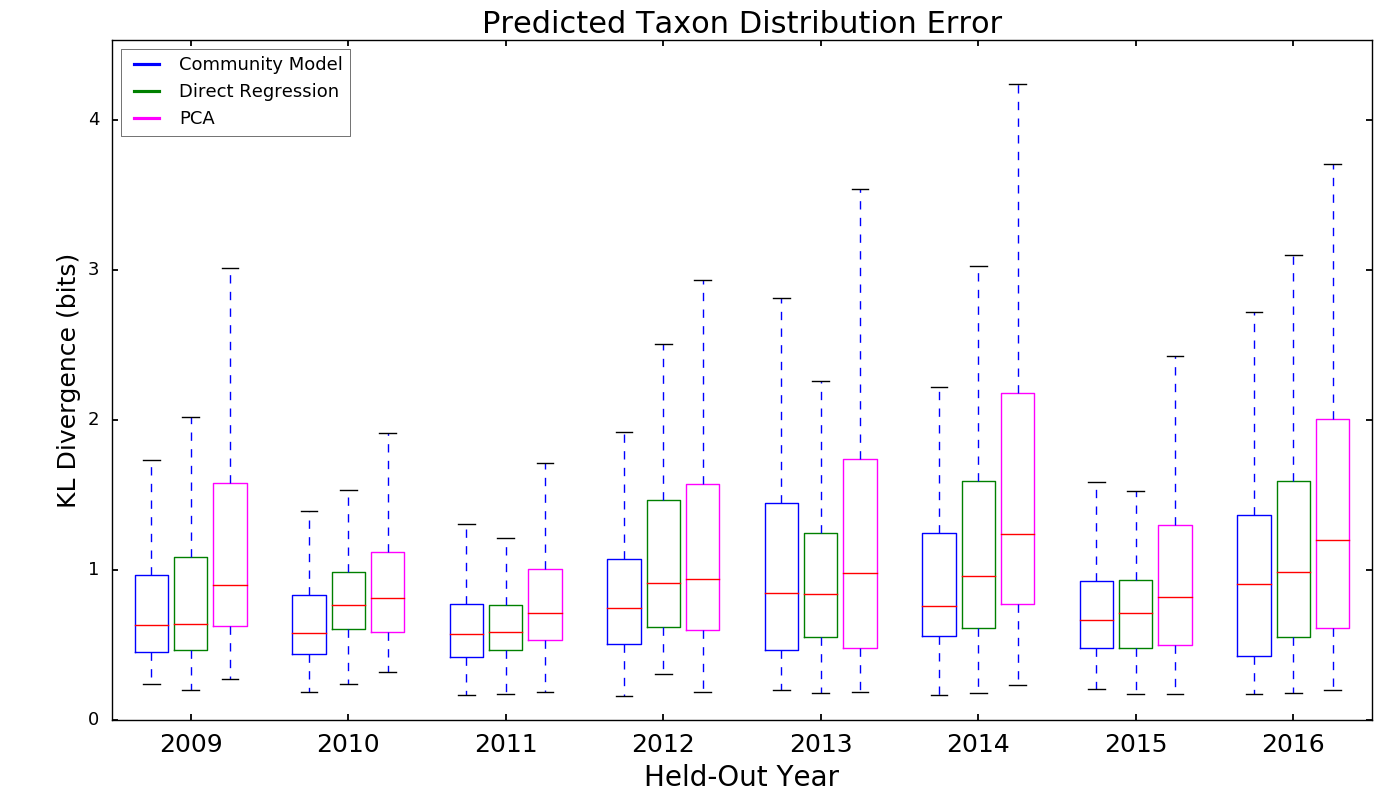
\includegraphics[width=0.8\linewidth]{figures/oceans/KLDivergenceBoxplot-C.png}
    \caption{Comparison of daily taxon distribution prediction divergences for each of the three regression methods and each of the years in the dataset. For each year, the other 6.5 years were used as training data. The community based regression method (ours, left) shows the lowest median KL-Divergence for all years.}
    \label{fig:plankton-mvco-kl-boxplot}
\end{figure}

We evaluated the resulting regression systems for all hyperparameter settings as well as the two baseline methods by comparing the predicted taxon distributions to the true distributions on each day in the dataset. Our error measure is the KL-Divergence between the predictions and the held-out distributons. We chose the community model hyperparameters settings with the lowest average KL-Divergence over all the days in the dataset, ultimately picking a model with 6 active communities. The predicted taxon distributions for this model are shown in Fig.~\ref{fig:plankton-mvco-word-est}.

Fig.~\ref{fig:plankton-mvco-kl-boxplot} shows the taxon distribution prediction errors for this community model and our two baseline models, broken out by year. The boxes represent the distribution of prediction errors for nearly 365 days in 2009 through 2015, and 172 days in 2016 (nearly 365 because of some small gaps in the taxon count data). Our community model (leftmost for each year) achieved the lowest median error on every year in the dataset. We found that by optimizing the hyperparameters for the regression task, we were able to choose an interpretable representation of the community structure. In contrast, PCA does not feature any prior for temporal smoothness. As a result although its prediction error is on average only a little less accurate than our model's, the sequences of predictions it makes are sometimes implausible, featuring taxon distributions that change much more rapidly than the observed data. We found that both baselines were extremely susceptible to noise in the environment data, on average performing better than expected, but occasionally making extremely poor predictions (Fig.~\ref{fig:plankton-mvco-timeseries}). With our model, the regression problem is of a lower dimensionality than for direct regression, and therefore less susceptible to overfitting. For this reason when both models are presented with the same small amount of training data, our model is more able to avoid large errors for new inputs unlike the training data.

\begin{figure}
    \centering
    \subfloat[]{
        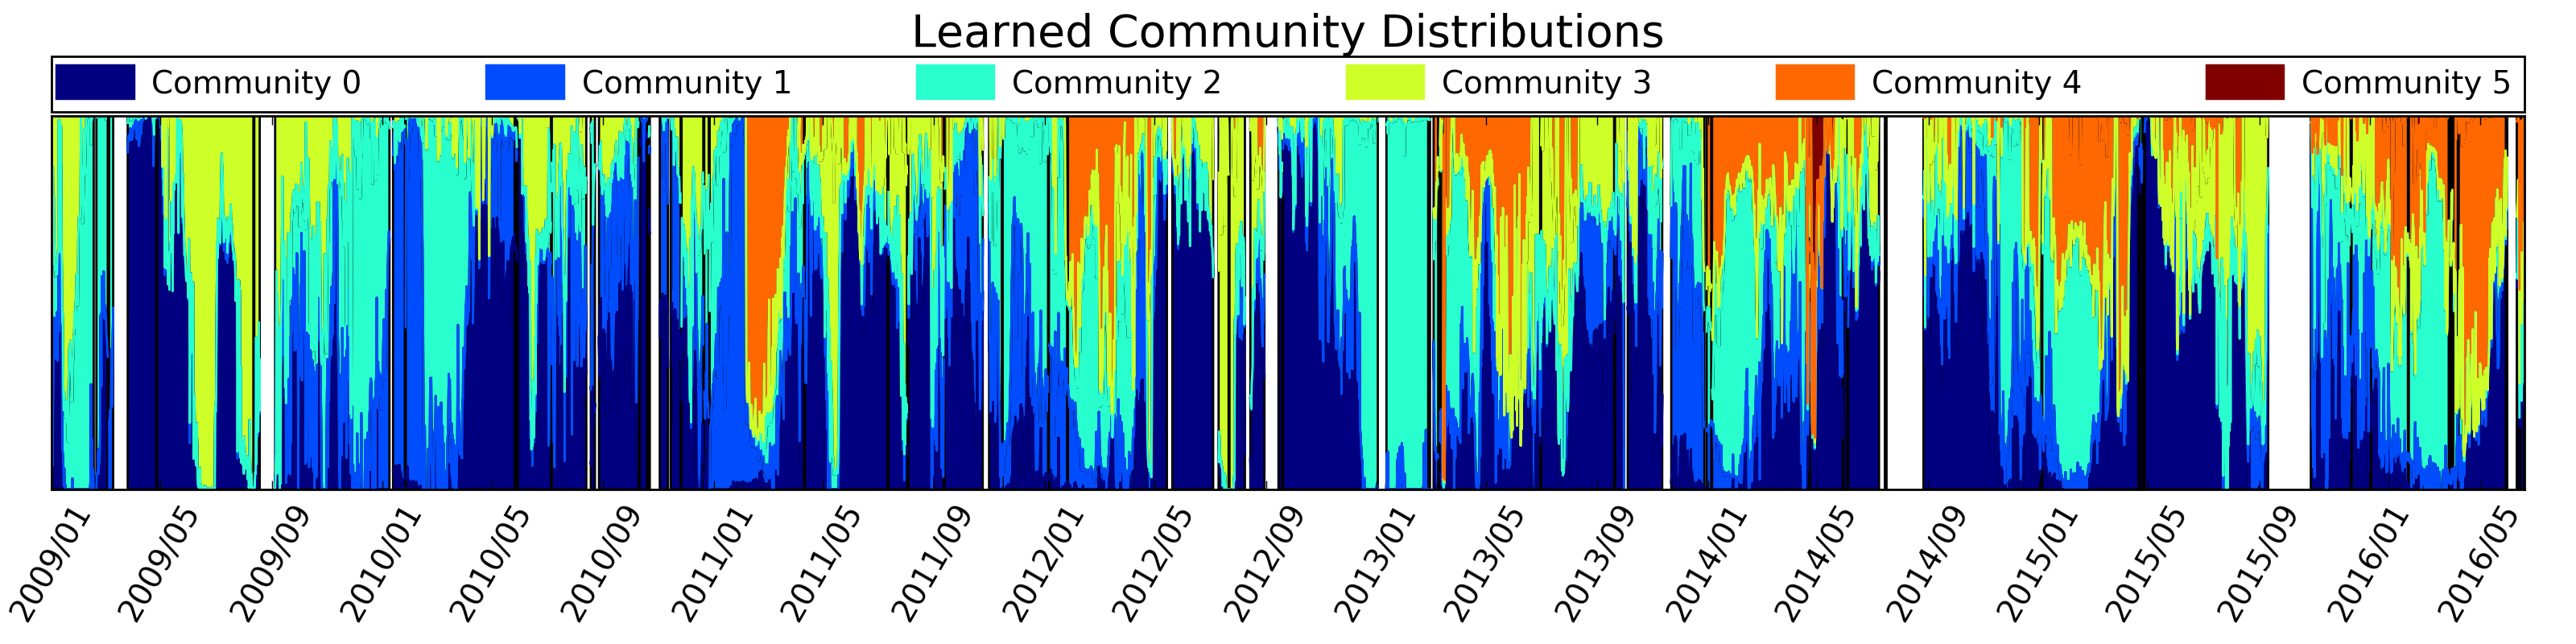
\includegraphics[width=\textwidth]{figures/oceans/theta_stacked.png}
        \label{fig:plankton-mvco-theta-stacked}
    }\\
    \subfloat[]{
        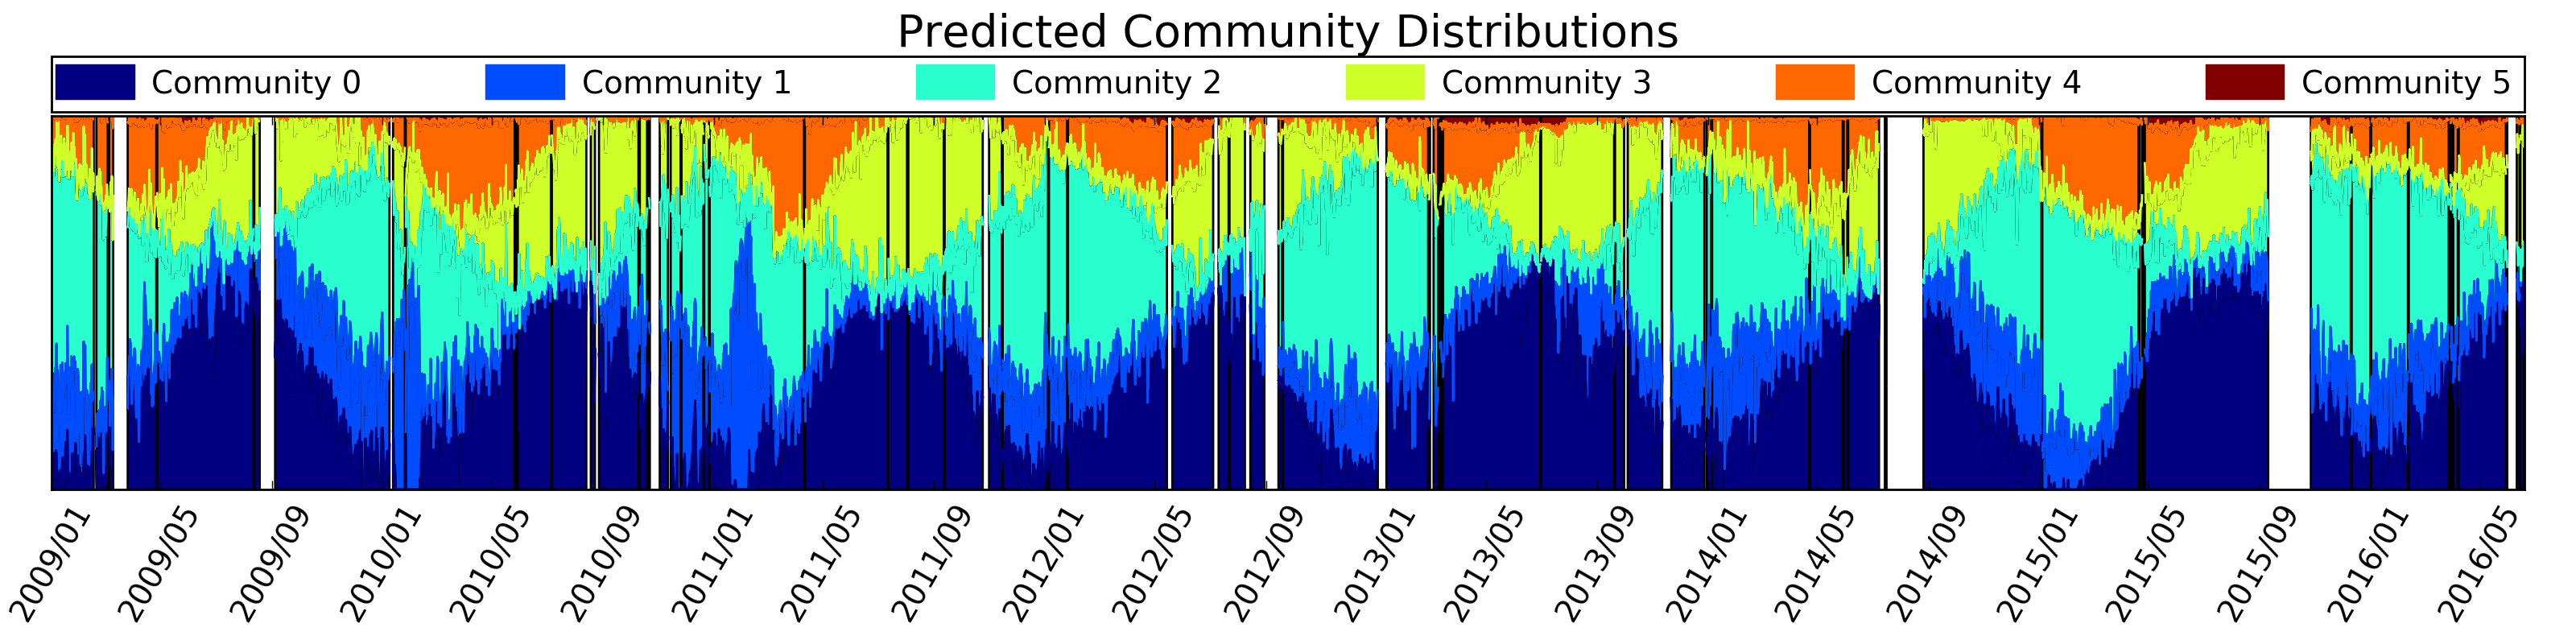
\includegraphics[width=\textwidth]{figures/oceans/theta_hat_stacked.png}
        \label{fig:plankton-mvco-theta-hat-stacked}
    }\\
    \subfloat[]{
        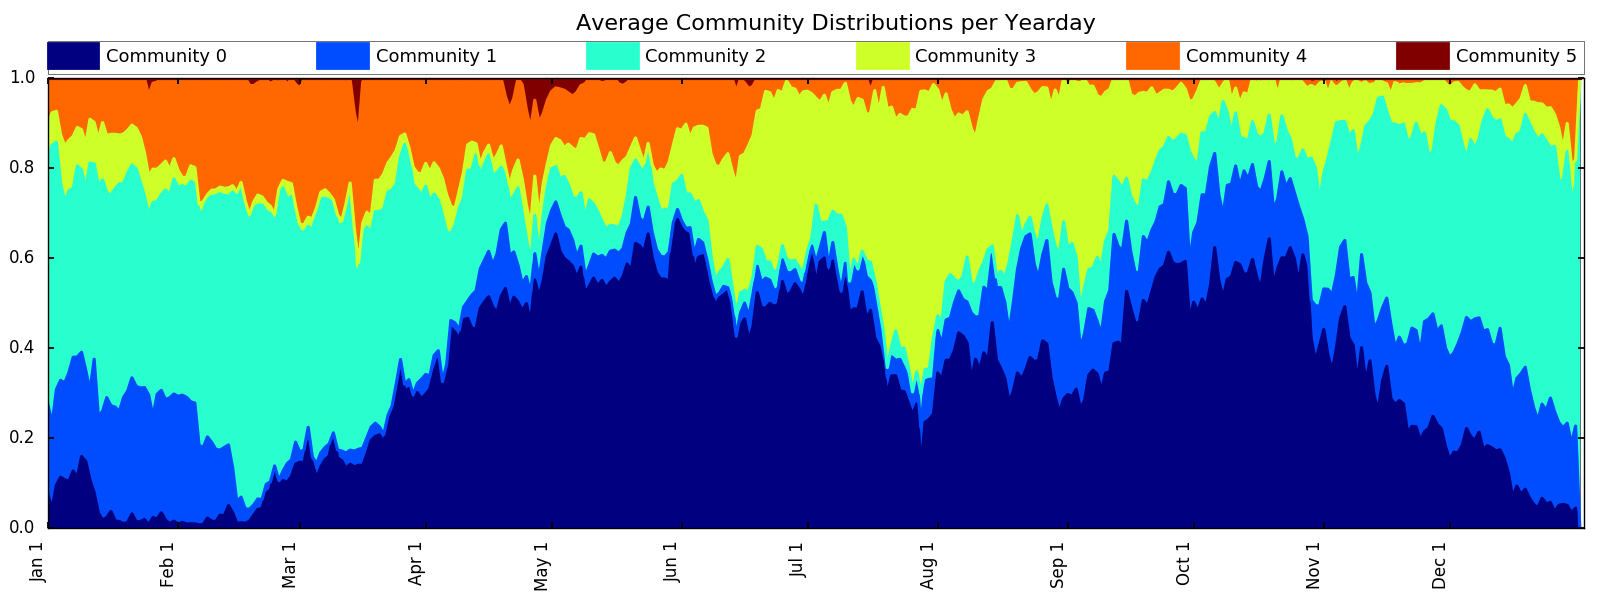
\includegraphics[width=\textwidth]{figures/oceans/theta_mod.png}
        \label{fig:plankton-mvco-theta-mod}
    }

    \caption{The learned and predicted community distributions. The horizontal axis represents time, and each community is represented by a color. The fraction of observations on a day belonging to a particular community are shown by the size of the colored area (totalling 1 for each day). Our model finds strong seasonal structure in the data without having such an assumption built-in.
    \protect\subref{fig:plankton-mvco-theta-stacked} Daily community distributions over 7.5 years for the best performing community model on the regression task.
    \protect\subref{fig:plankton-mvco-theta-hat-stacked} Daily community distributions predicted from environment data.
    \protect\subref{fig:plankton-mvco-theta-mod} Average community distribution for each day of the year over the entire dataset.
    }
    \label{fig:plankton-mvco-theta}
\end{figure}

An intriguing result of our community regression model is that nearly all of the magnitude in the weights of the learned regression parameters is either on the day of the year, the water temperature, or the number of plankton classified for a given day (Fig.~\ref{fig:plankton-mvco-weights}). 
From our regression matrix, we can see that 5 out of 6 communities has a seasonal niche with which most stongly predicts its presence. We found that the best performing community models showed strong seasonal structure, rather than relying on other variables. This is made evident by the average community distribution for each day of the year over the entire dataset before regression (Fig.~\ref{fig:plankton-mvco-theta-mod}). Note that there are many possible community decompositions, and although our model makes weak assumptions about the temporal smoothness of the communities, it does not have any prior knowledge of the seasonal nature of the data. By performing hyperparameter optimization over the downstream regression task, we were able to select a model with just the right level of sparsity and temporal smoothness to emphasize this seasonal aspect and describe the data in an interpretable way.

\begin{figure}
	\centering
	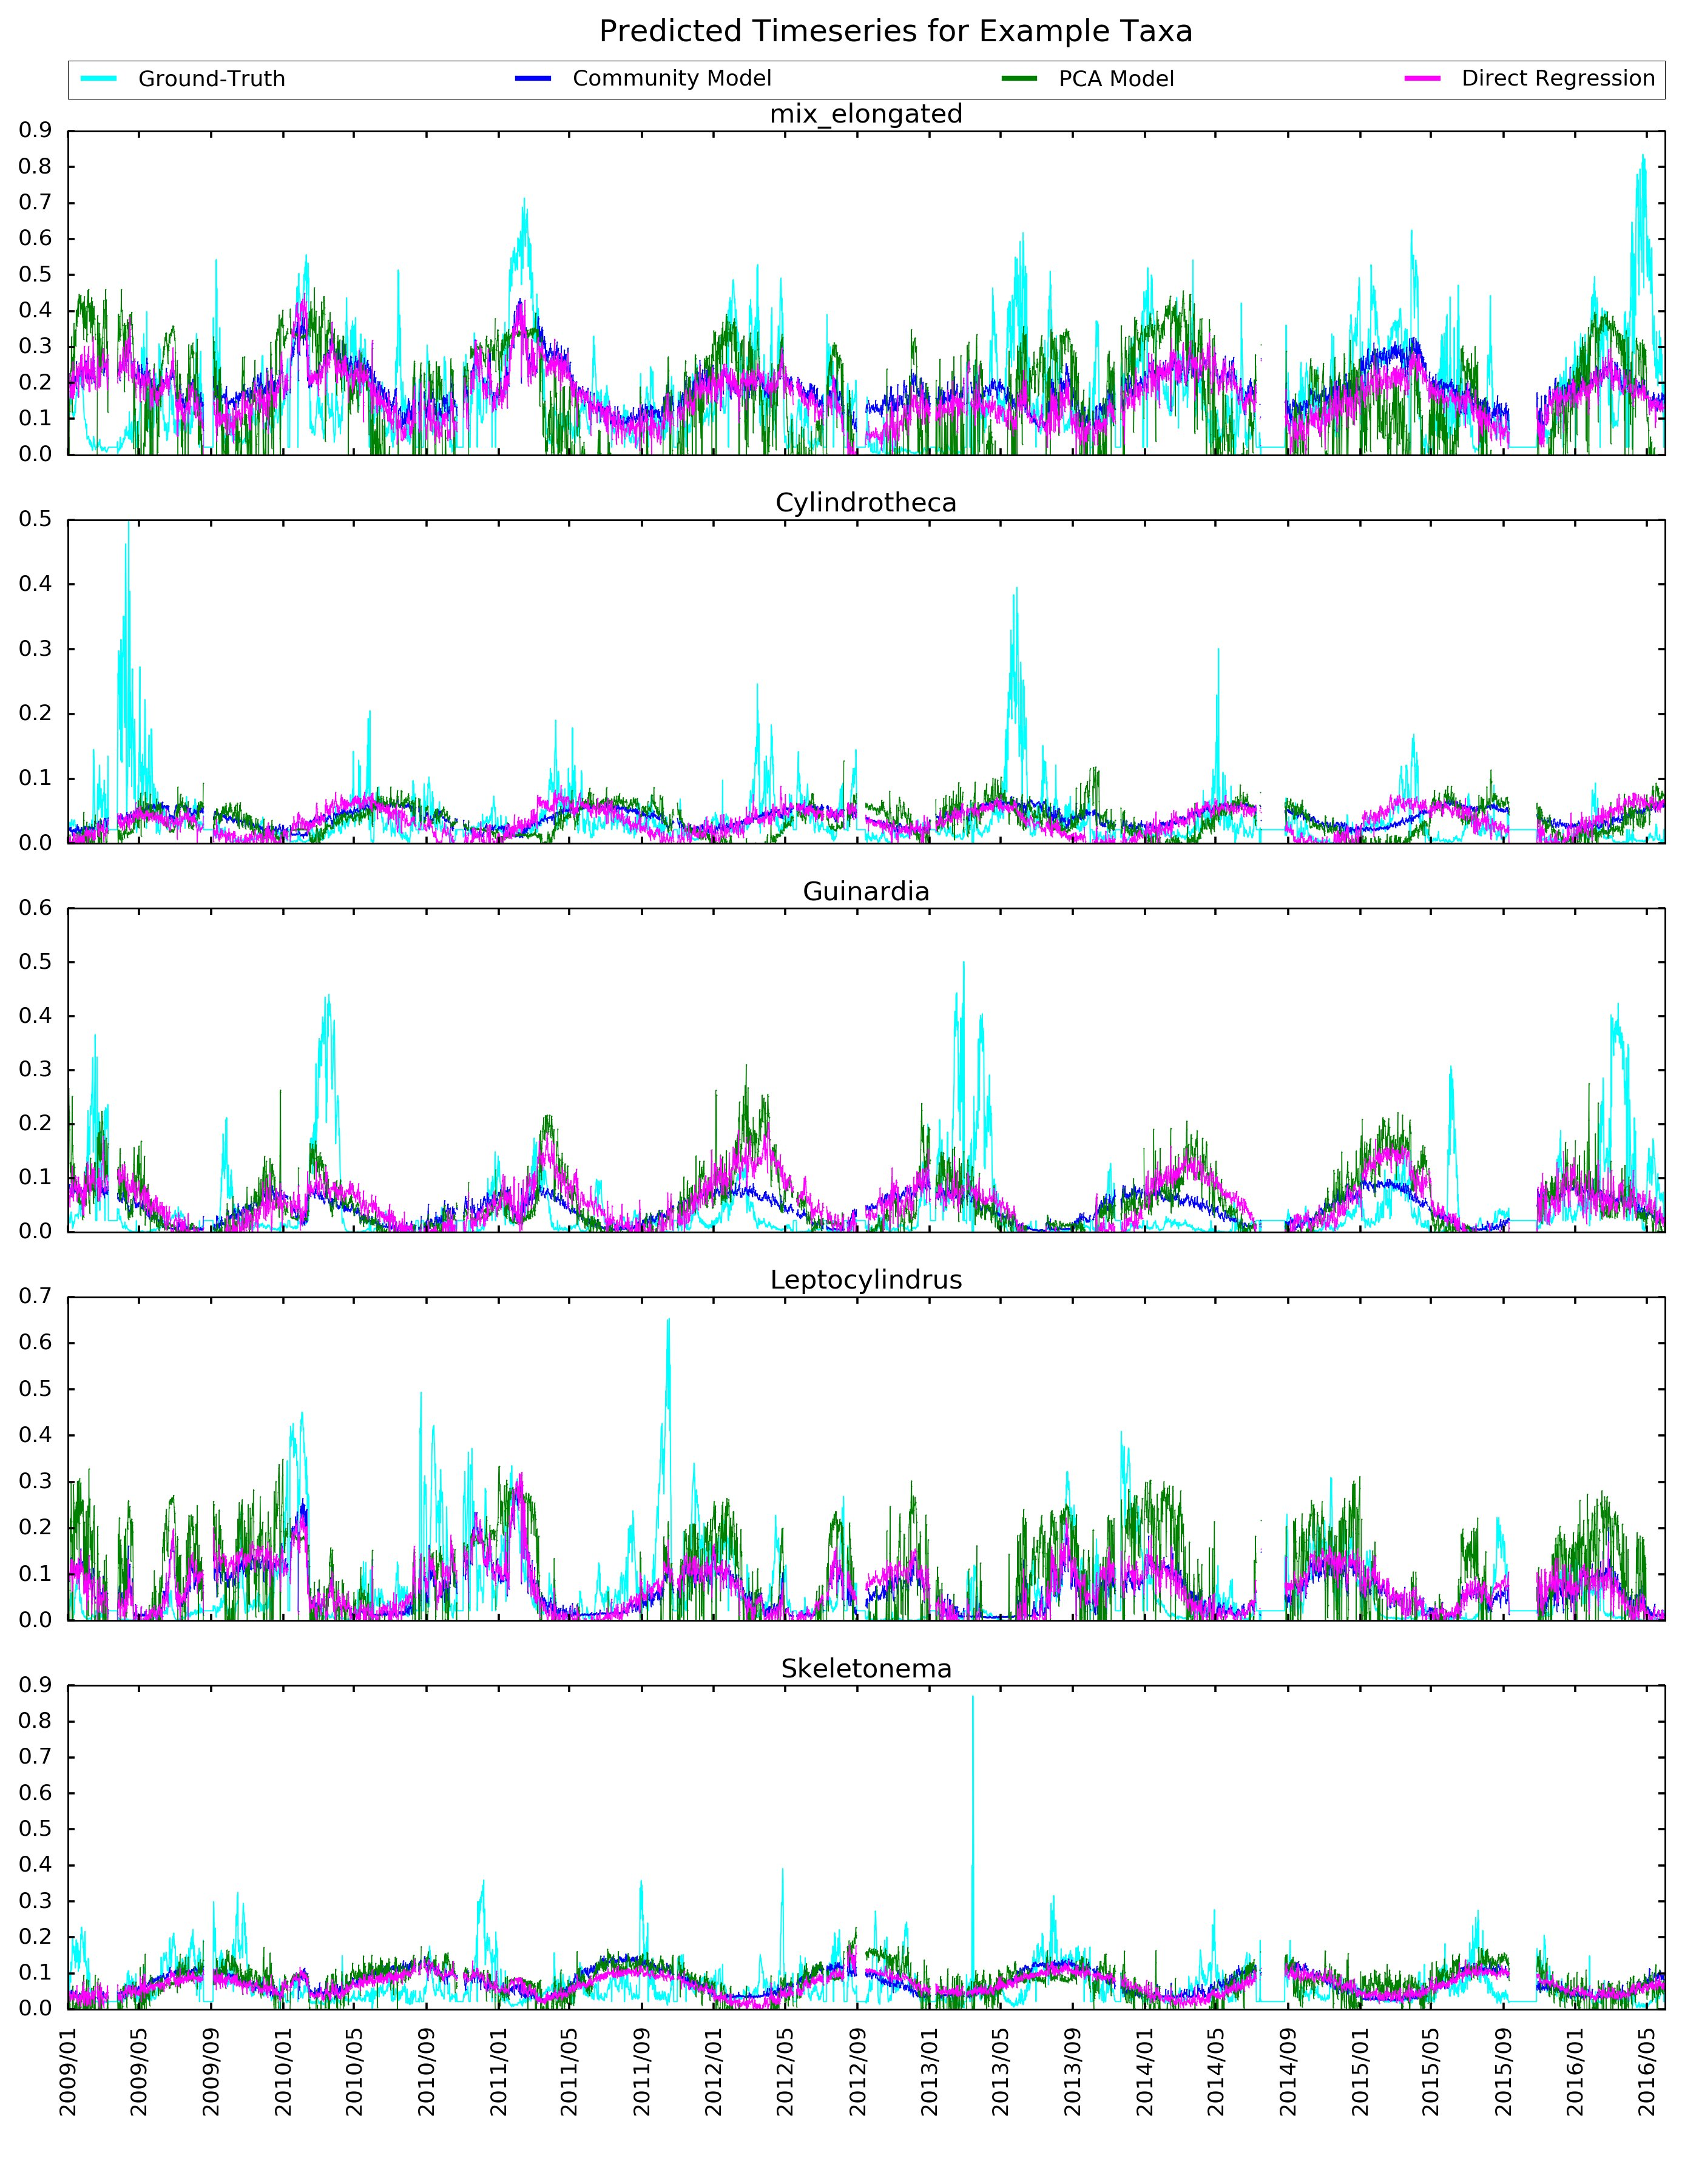
\includegraphics[width=0.95\textwidth]{figures/oceans/timeseries.jpg}
	\caption{Timeseries representation of individual probability of observing 5 common taxa on each day in the dataset. Note that the community model's predictions are less susceptible to noise that the other two strategies.}
	\label{fig:plankton-mvco-timeseries}
\end{figure}

Another outcome of our experiment is the communities themselves learned by our model (Fig.~\ref{fig:plankton-mvco-phi}). We found that across different hyperparameter choices, the top few most active communities were relatively similar to those presented here. Some associations based on our model have ready explanations. For instance community 1 is dominated by the taxa ``mix\_elongated'', representing miscellaneous centric diatiom chains, and ``leptocylindrus'', which both exhibit elongated morphologies and easily confuse the IFCB's vision-based classification system. As a more exciting example, communities 2 and 4 are the only communities with significant probability of observing the taxon ``Guinardia'', and are predicted by warm water temperatures, while \emph{Guinardia delicatula} populations have been noted to be negatively associated with parasites that do not survive during cold winters \citep{peacock2014parasitic}.

\begin{figure}
    \begin{center}
        \subfloat[]{
            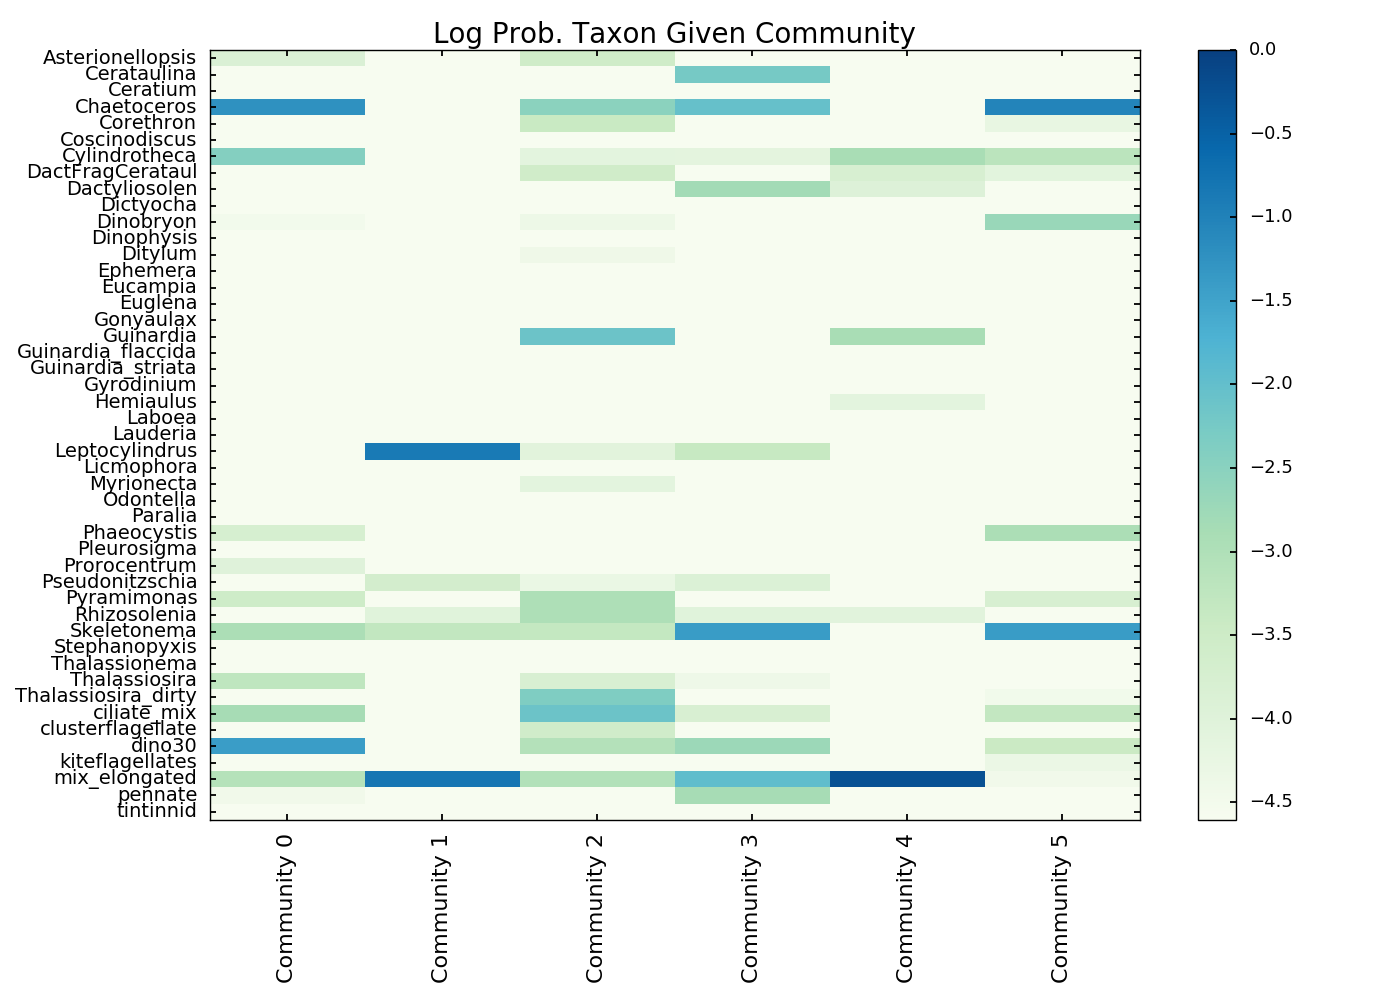
\includegraphics[width=0.49\columnwidth]{figures/oceans/LogPhi.png}
            \label{fig:plankton-mvco-phi}
        }%
        \subfloat[]{
            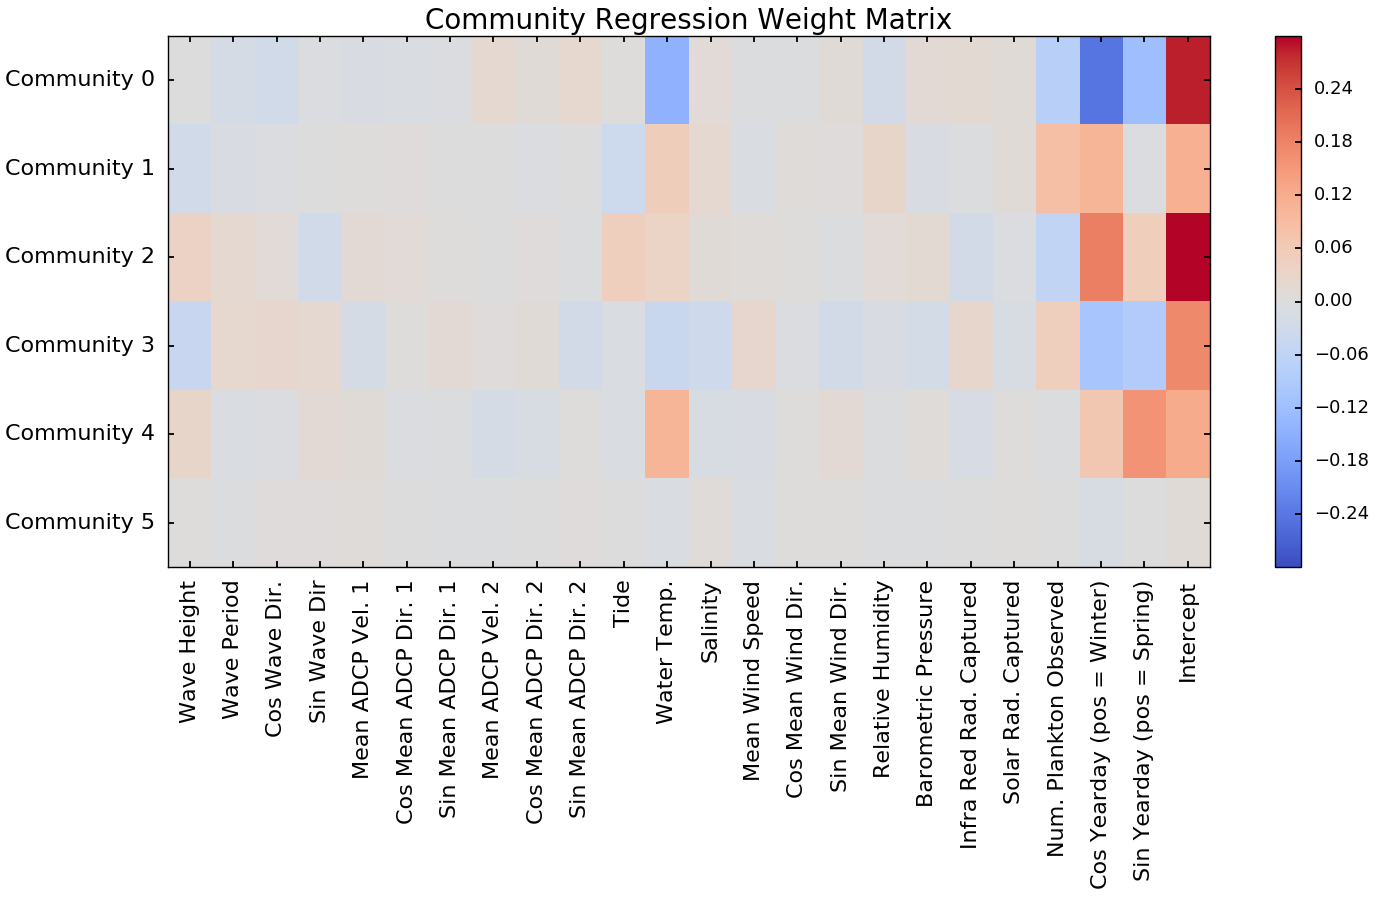
\includegraphics[width=0.49\columnwidth]{figures/oceans/weights.png}
            \label{fig:plankton-mvco-weights}
        }
    \end{center}

    \caption{
        \protect\subref{fig:plankton-mvco-phi} Log-probability of each taxon for each community.
        \protect\subref{fig:plankton-mvco-weights} Linear regression weight matrix for top-performing community model.
    }
    \label{fig:plankton-mvco-supplemental}
\end{figure}

Our community model takes a complex, high-dimensional population dataset, and offers immediate questions to pursue related to the ecology of specific taxa near MVCO. For instance, in Fig.~\ref{fig:plankton-mvco-theta-stacked} we see that community 4 begins to appear a little earlier each year from 2011, at first appearing only in the spring, and by 2015 persisting throughout the Winter. If we were to only look at the timeseries for the individual taxa, ``mix\_elongated'', ``Guinardia'', and ``Cylindrotheca'' which dominate community 4, this pattern is not obvious at all (See Ground-Truth, Fig.~\ref{fig:plankton-mvco-timeseries}). However, our model highlights that these taxa often co-occur, and that the pattern of co-occurrence shifts over the years.

\section{Predicting presence of missing phytoplankton by their associates} \label{sec:plankton-spatial-search}
In our second study of IFCB plankton data, we ground our community model by its ability to predict the presence of an artificially held-out plankton taxon from the others, rather than predicting the full distribution from auxillary data \citep{Kalmbach2017a}. Further, in this application we explore spatial phytoplankton classification data, demonstrating our model's ability to capture both the temporal and spatial smoothness aspects of community structure.

This work is motivated by a scenario where a plankton ecologist is searching for a particular plankton taxon. If the ecologist deploys IFCB on a ship and periodically collects samples, but never observes the taxon of interest, she requires further information to decide whether to move on or keep collecting samples in the same location. Because IFCB samples are a small volume of water, yet ecologists would like to describe large volumes of ocean that have complex ecosystems, it is very likely that samples will sometimes be deficient in taxa that are, in fact, found near the sample location. Therefore, we propose to model the associations between taxa in such a way that if we disregard the target taxon we can still estimate the community mixture for a location accurately, and consequently predict the presence or absence of the target from its known assocaites.

We would like to estimate the probability of observing a falsely-missing target taxon $v^\star$, based on the observed distribution of the $V-1$ other taxa.
We assume that the taxon is not systematically missing, in other words that we can collect a training set at some other locations comprised of all $V$ taxa.
Then given this training set, we learn the topic assignments and MLE priors $\hat{\Theta}$ and $\hat{\Phi}$. At test-time we disregard the target taxon, assuming it is falsely-missing. To address this we consider the topics excluding $v^\star$ as the maximum likelihood of the Dirichlet posterior over the other $V-1$ taxa. In other words, at test time we use topics which ignore the missing taxon:
\begin{equation}
P(w = v | z = k, \boldsymbol{w}) \approx \hat{\Phi}_k^{-v^\star} \triangleq \frac{N^{w_i}_k + \beta}{\sum_{u \neq v^\star} N^u_k + \beta},
\end{equation}

Next, we obtain topic assignments $\boldsymbol{z_{- v^\star}}$ by substituting $\hat{\Phi}_k^{- v^\star}$ for $\Phi$ in the predictive distribution Eqn.~\ref{eqn:posterior}. In the iterative process of sampling topic assignments, we fix $\hat{\Phi}_k^{-v^\star}$, and only update topic assignments for \emph{new} observations based using the `target defficient' topic assignment counts. These define the approximate MLE topic priors $\check{\Theta}_{g(x)}$. Finally, we estimate the proportion of the data which would have been made of the target class using the original MLE topic matrix
\begin{equation}
P(w_x = v^\star | \mathbf{w}_{-v^\star}) \approx \sum_{k=0}^K \check{\Theta}_{g(x),k} \hat{\Phi}_{k,v^\star}
\end{equation}

\subsection{US Atlantic coast hotspot prediction experiment}

We demonstrate this approach with IFCB classification results from NOAA's Fall 2014 EcoMon Survey aboard the Research Vessel Pisces (Cruise PC 14-05). The IFCB was configured to automatically sample from underway flowing surface seawater during the period 4-19 November 2014. The classification system generated over 140,000 individual phytoplankton observations from these water samples. Classification results comprise a dataset with 47 taxa at 852 locations spanning the US Atlantic coast from North Carolina to Maine (See Fig.~\ref{fig:plankton-pisces-summary-in}).

\begin{figure}
	\centering
	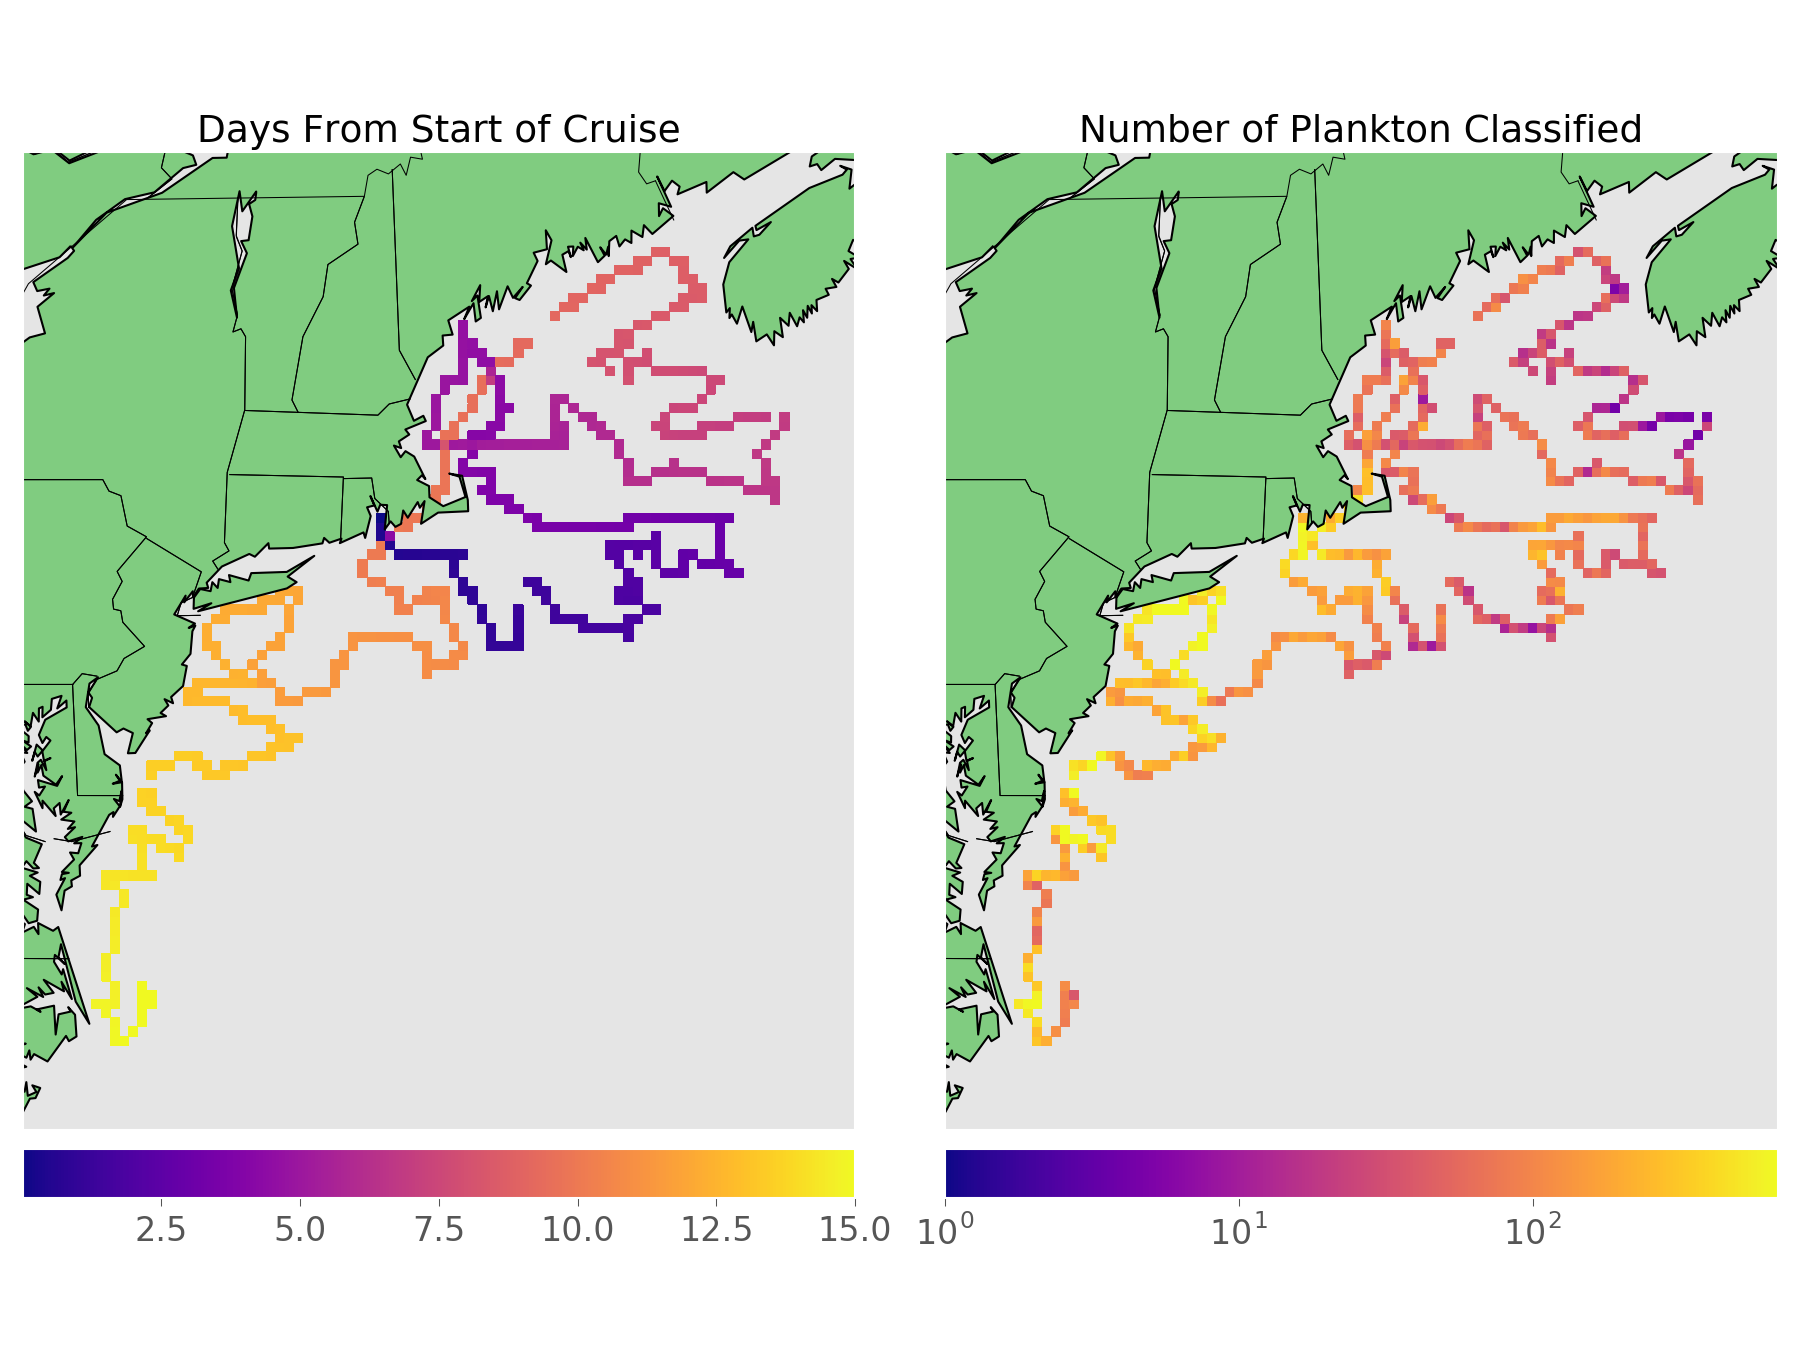
\includegraphics[width=0.75\textwidth]{figures/icra_plankton/n_plankton.png}
	\caption{Summary of data recorded during the Pisces 14-05 cruise. Left, color shows progress in time. Right, color shows the number of plankton observed at each sample location.}
	\label{fig:plankton-pisces-summary-in}
\end{figure}

We divide the sample locations into equal-sized parts, representing the training and test phases of the simulated mission. The counts of all 47 taxa were kept in the training set and used to learn the topic model. For the test set, we held out each of the 8 most-frequently observed phytoplankton taxa one at a time. We define the hotspots of
a taxon to be the top 50 sample locations in the test data, where the relative abundance of the taxon to all other taxa was highest. The 8 tested taxa make up just over 81\% of all the observations in the dataset. The most common taxa are miscellaneous centric diatom chains (``mix\_elongated''), mixed species of pennate diatoms, \emph{Thalassiosira} spp., \emph{Guinardia delicatula, Guinardia striata, Dictyocha} spp., \emph{Ephemera} spp., and \emph{Phaeocystis} spp. While our method accounts for the sparsity of taxon distributions, this dataset also features sparsity in terms of the locations of observations. To address this separate issue, we resort to a 2D spatial median filter. Finally, we apply a threshold to identify the hotspot locations.

We compared our method to an exhaustive search strategy and a k-means search strategy. For each sample in the test set, exhaustive search estimates the probability of observing $v^\star$ by looking up the sample in the training set with the most similar distribution to the observed data. This represents the strategy which makes the most use of all the data available for every test sample, at the cost of a linear computational complexity in the number of sample locations in the dataset. In the k-means strategy, we fix a constant test-time complexity by reducing the search space to the $K$ centroids returned by a standard k-means clustering implementation. These centroids are defined such that if each class distribution in the training set were replaced by the nearest of the $K$ centroids, the sum of squared error is approximately minimized, however it does not take into account the sparsity or spatial smoothness of the underlying distributions.

We carried out experiments for two different train/test regimes. First, we used every second sample location for training (see Fig.~\ref{fig:plankton-pisces-maps-8}, column 1). This regime simulates a mission where the classifier frequently fails to identify examples of a class, for instance because its classifier was poorly tuned. Because nearby sample locations tend to have similar distributions, this regime tests the ability of a model to interpolate over small distances. Second, we used the first half of the sample locations as training (Fig.~\ref{fig:plankton-pisces-maps-1}, column 1), and the second half for testing. This latter case simulates a mission where the capabilities of the classifier have changed from the first half to the second half. It tests the ability of a model to predict in a new location that is not likely to have any spatially linked correlation with the training data.

\begin{figure}
    \centering
    \resizebox{0.9\textwidth}{!}{%
        \begin{tabular}{c}
        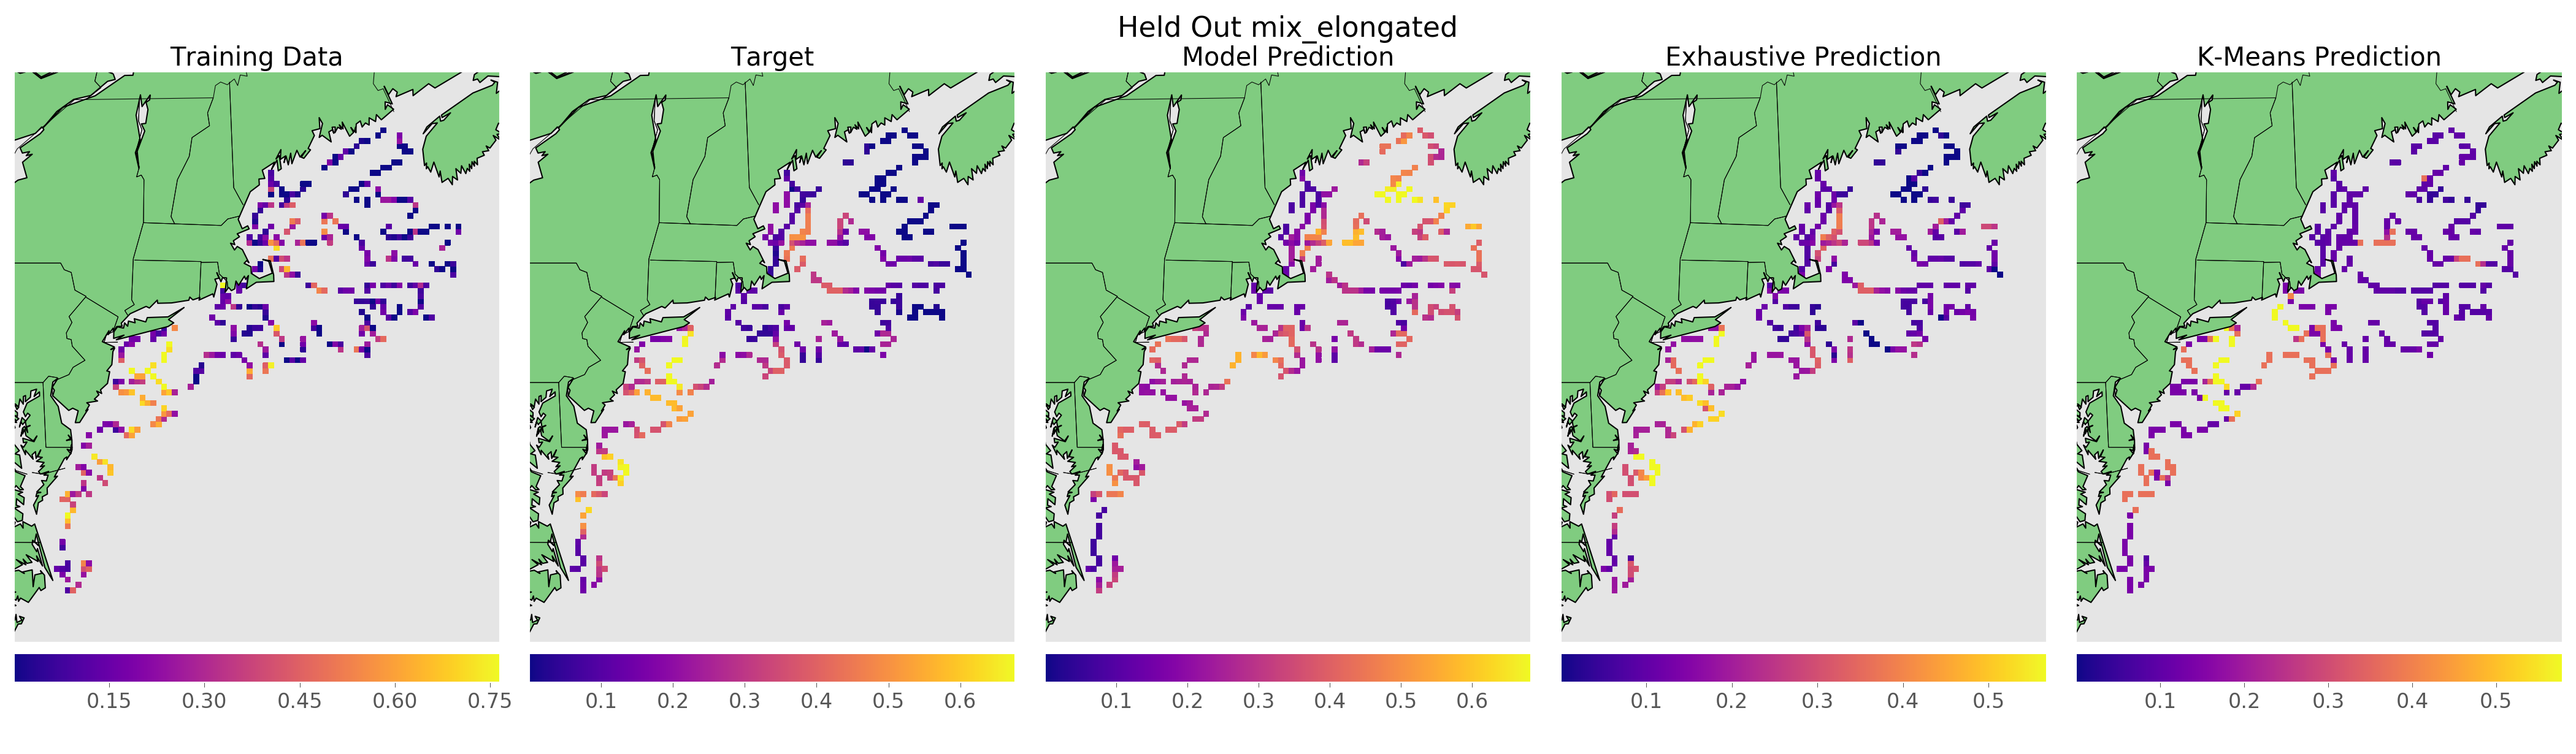
\includegraphics{figures/icra_plankton/maps_mix_elongated_8} \\
        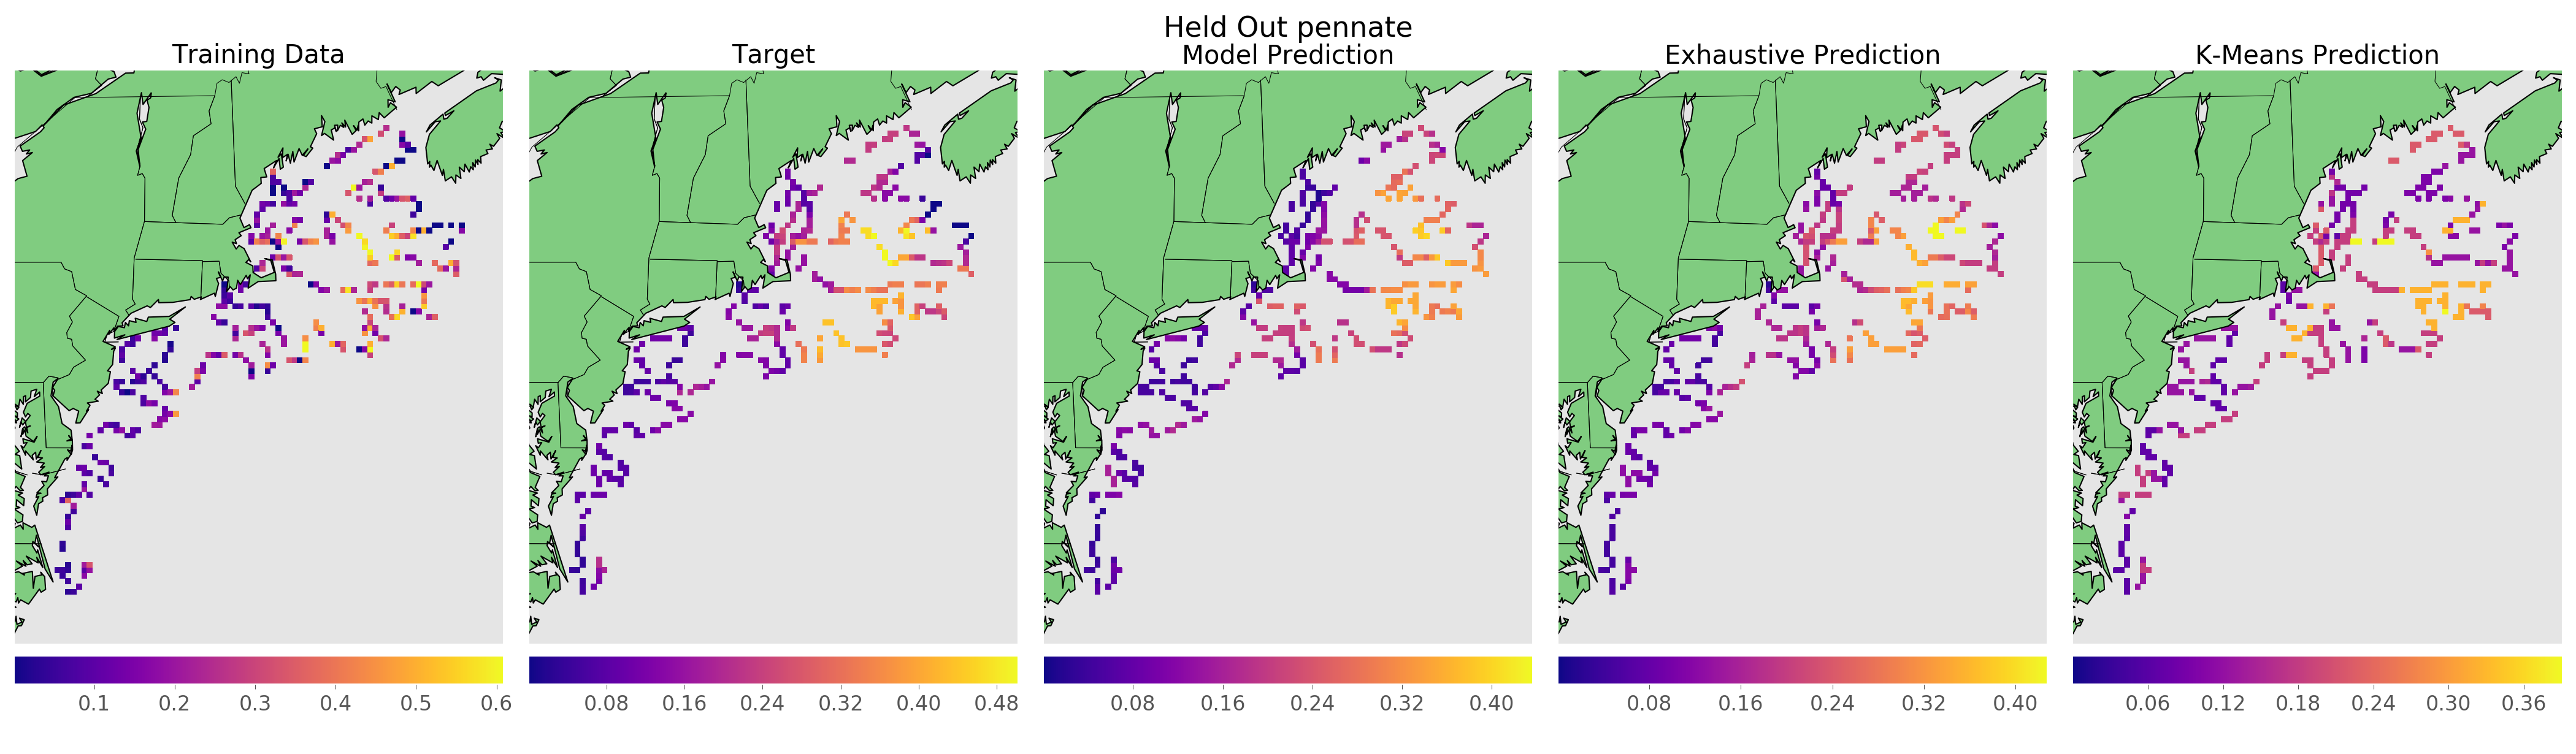
\includegraphics{figures/icra_plankton/maps_pennate_8}\\
        +
        %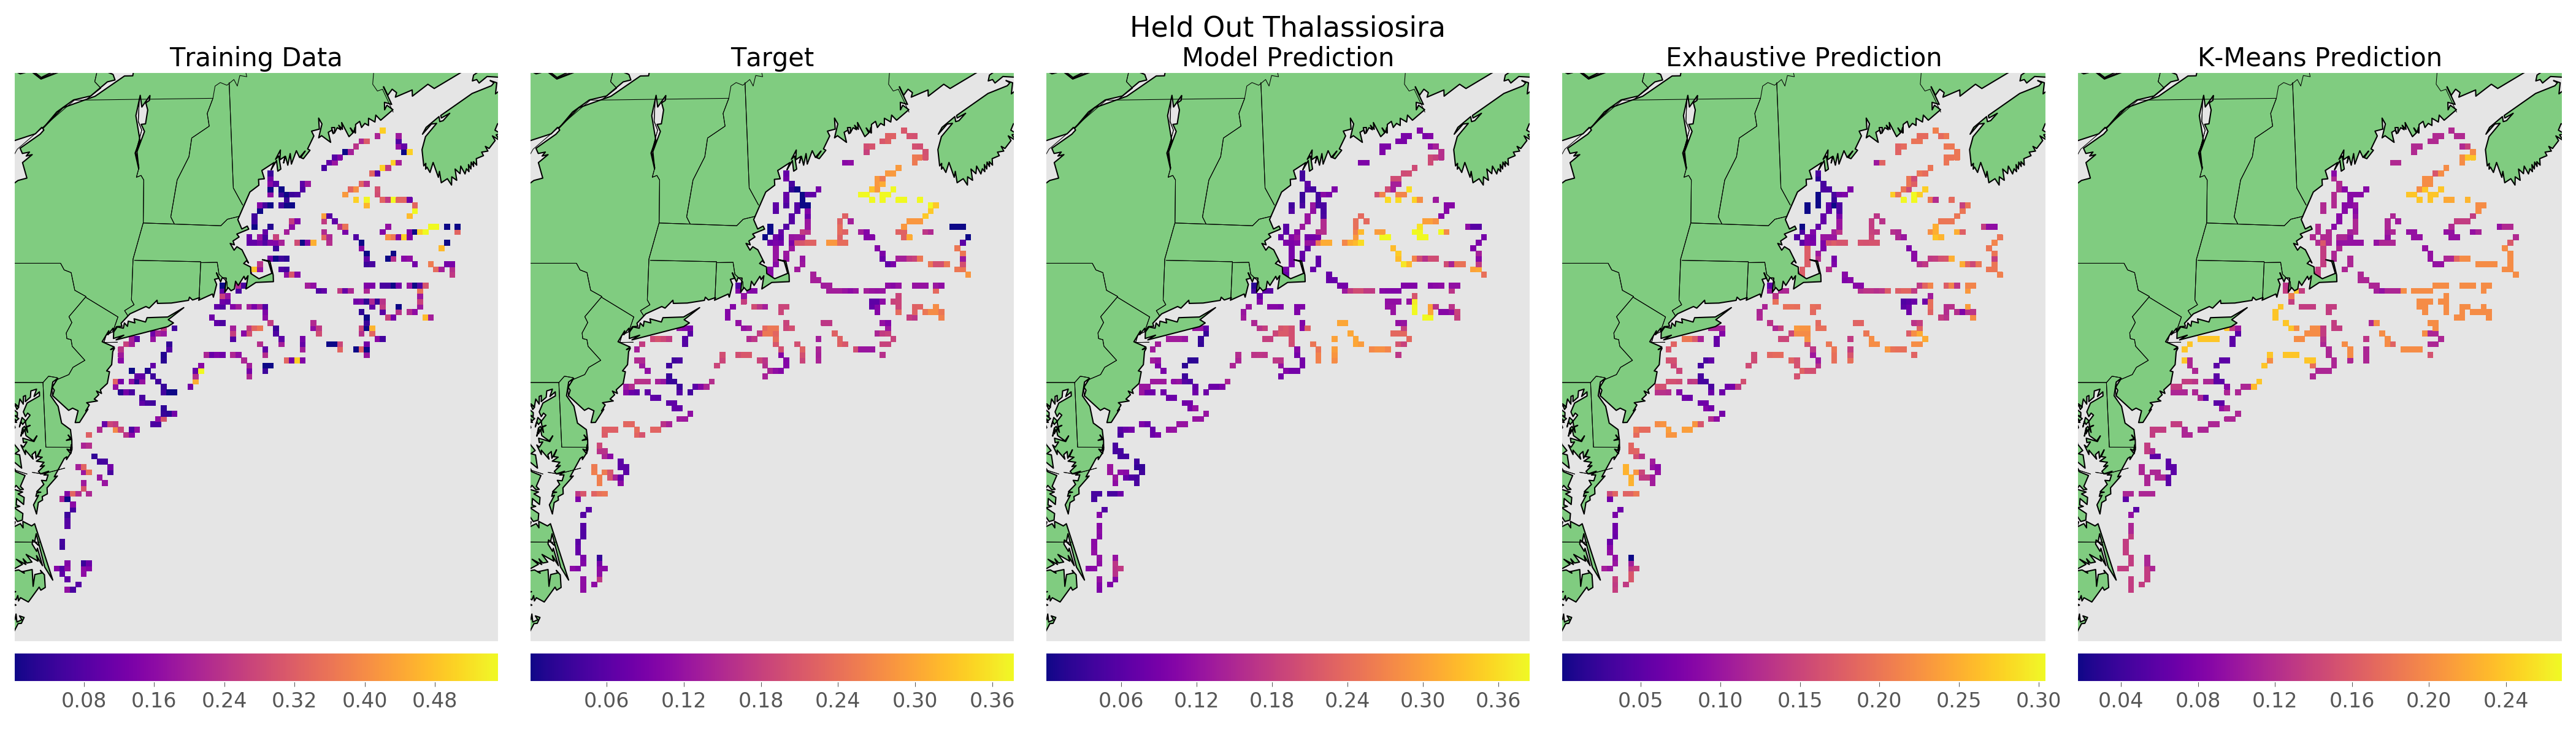
\includegraphics{figures/icra_plankton/maps_Thalassiosira_8}\\
        % 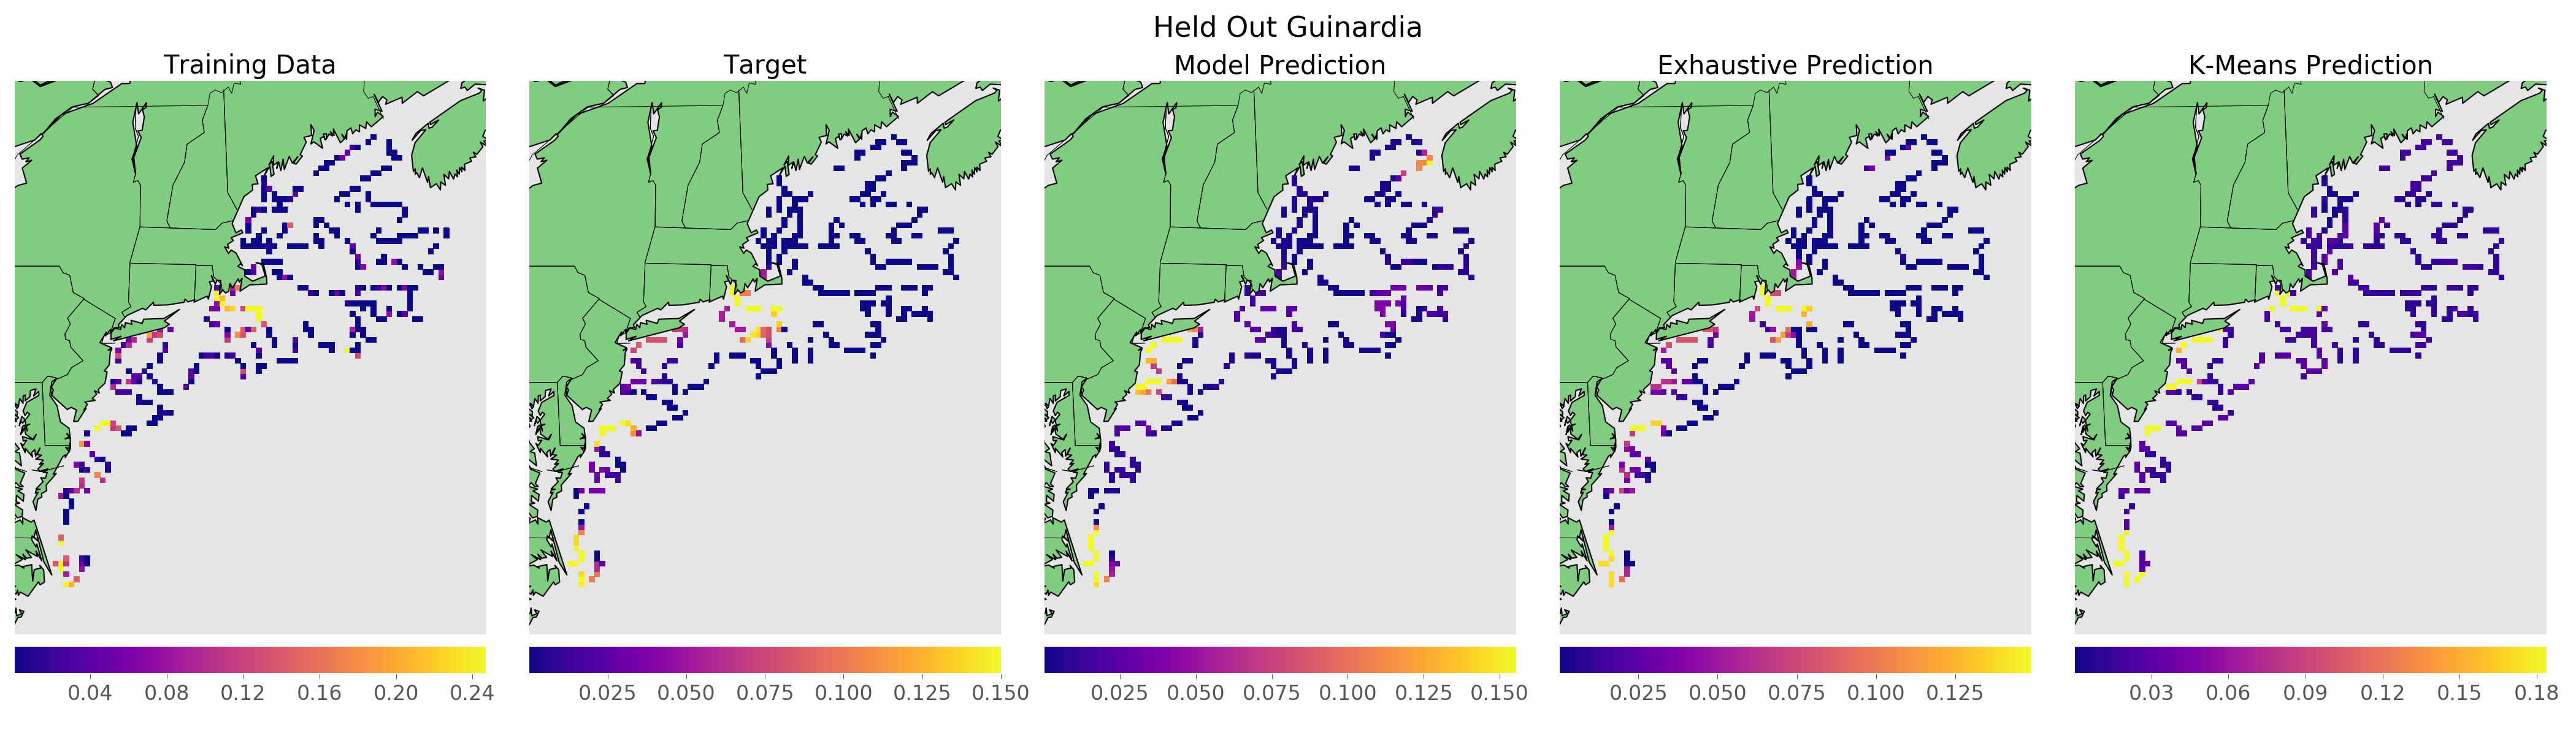
\includegraphics{figures/icra_plankton/maps_Guinardia_8}\\
        % 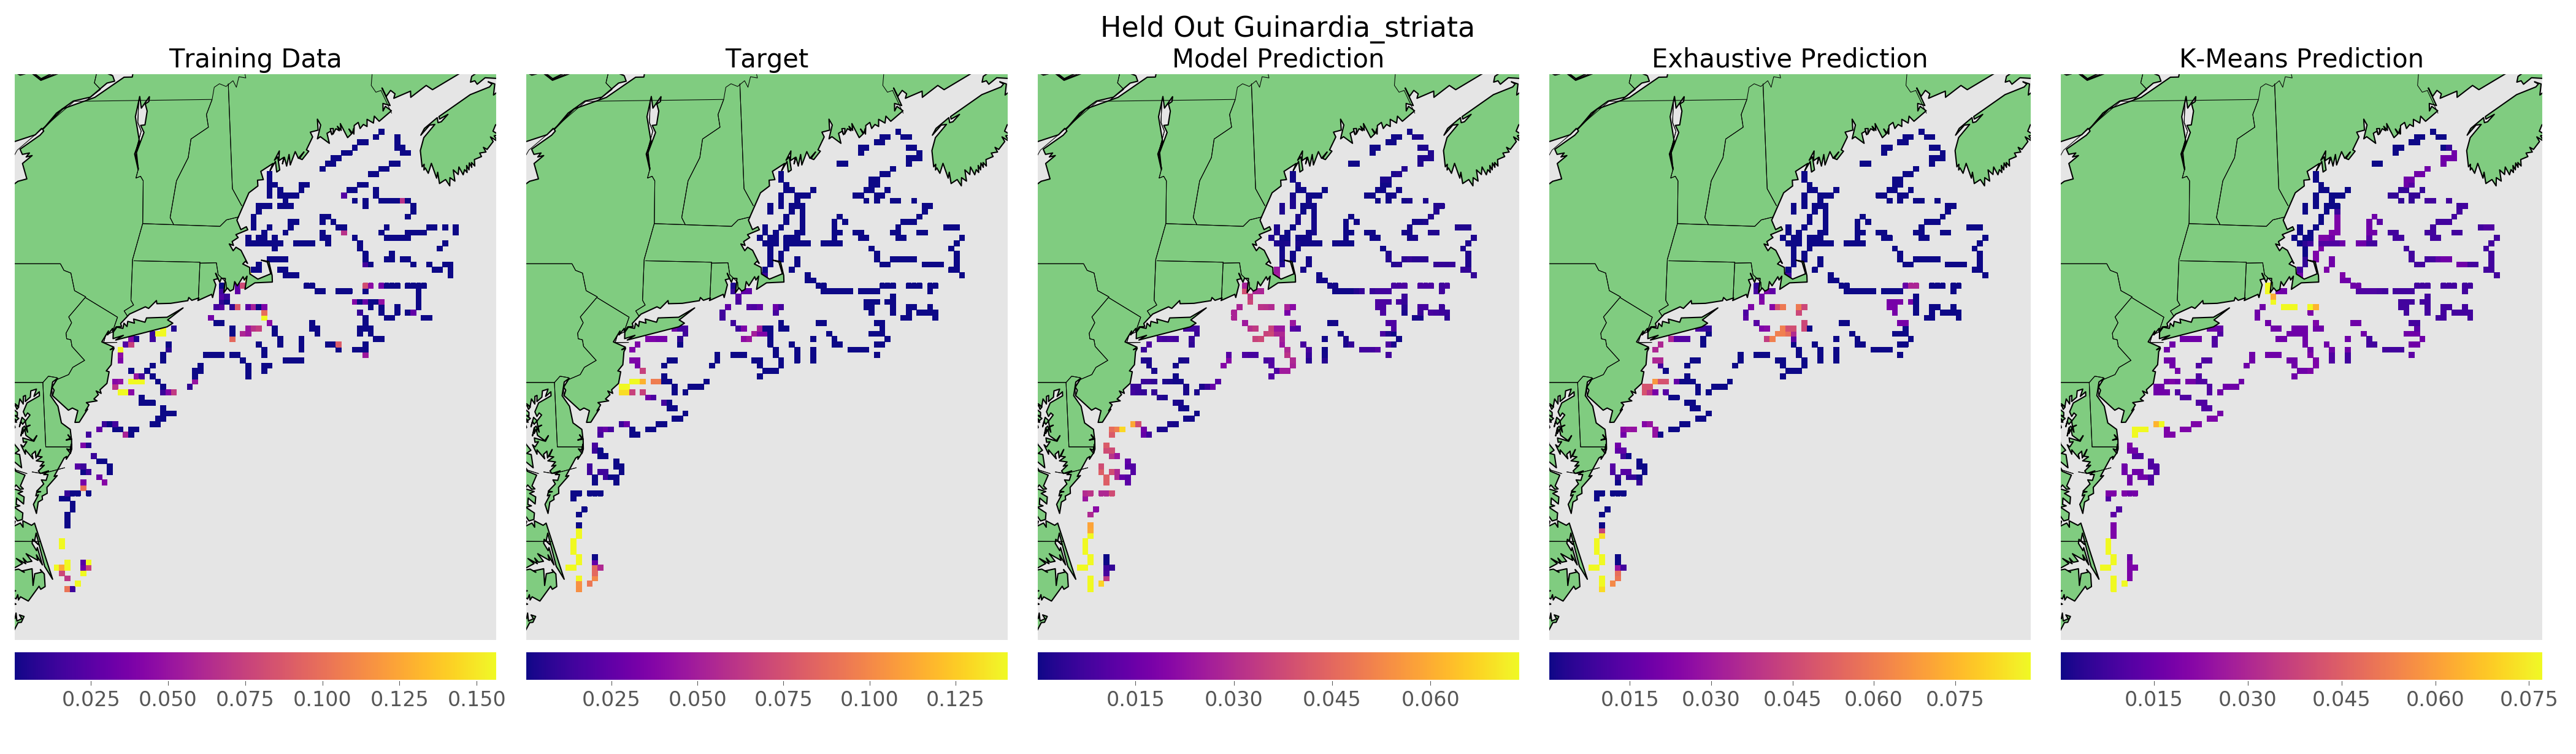
\includegraphics{figures/icra_plankton/maps_Guinardia_striata_8}\\
        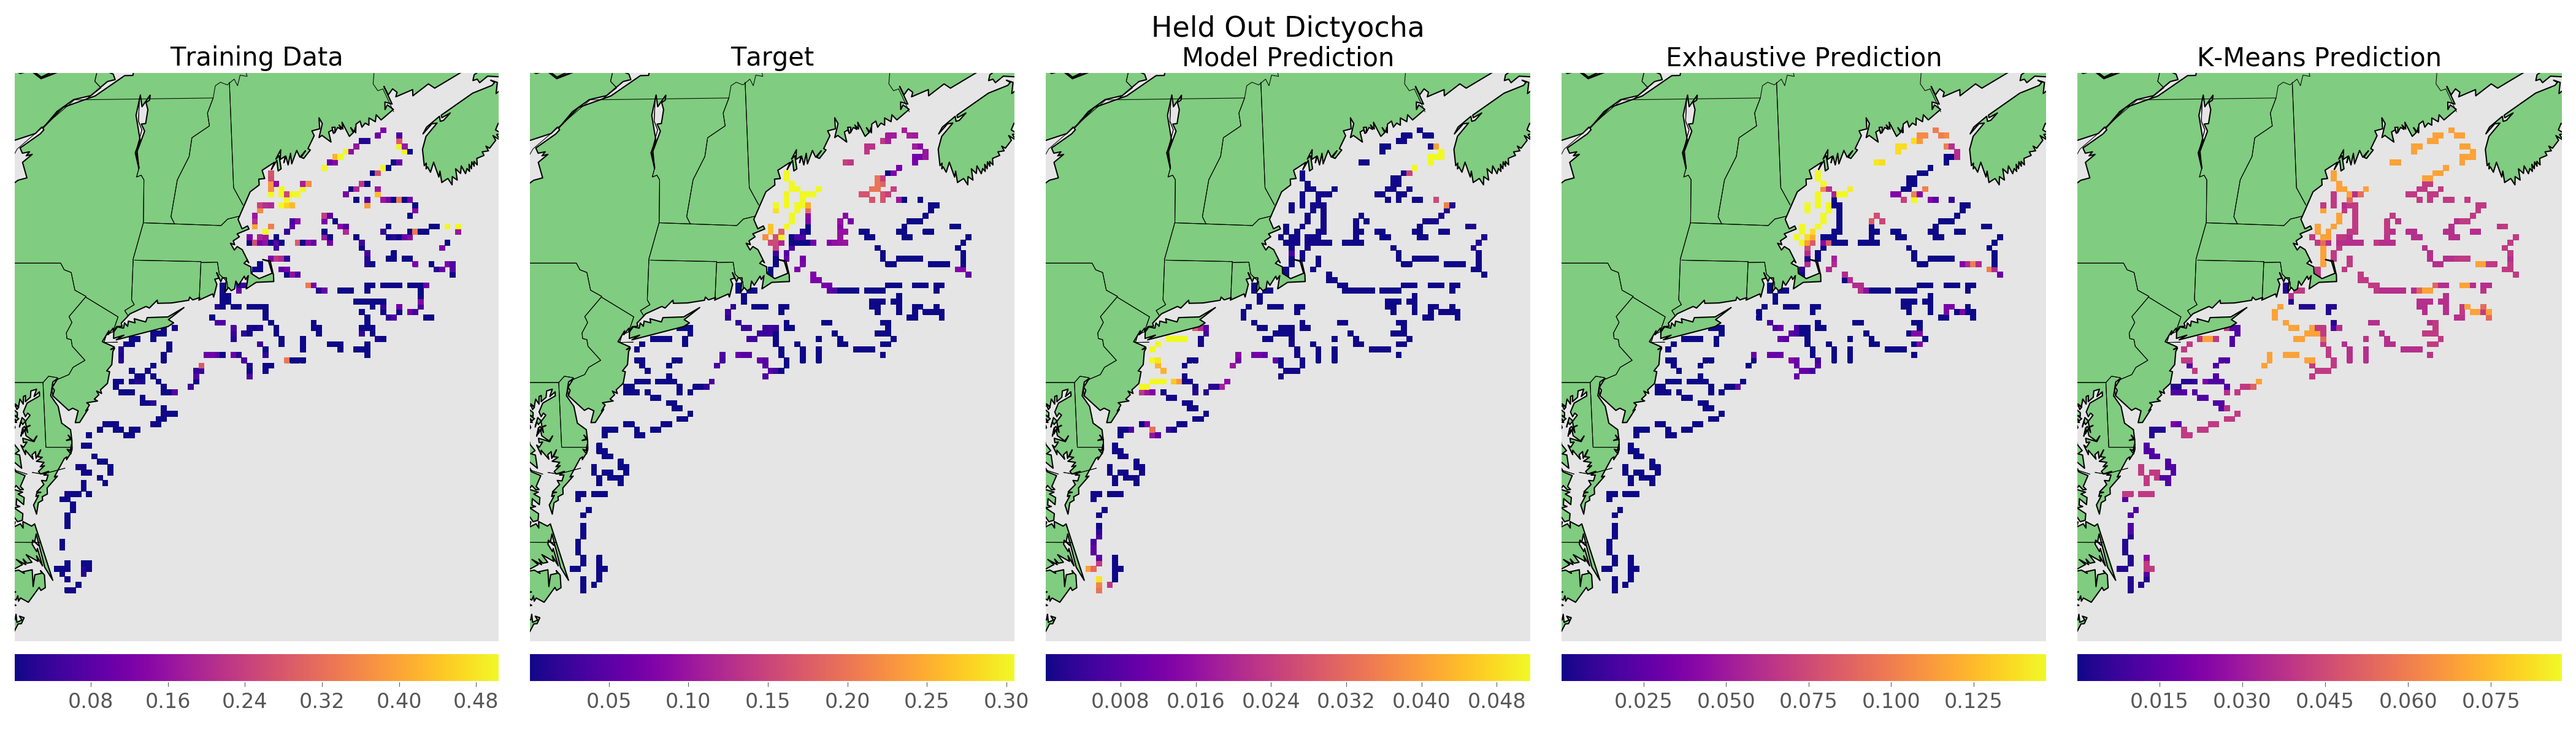
\includegraphics{figures/icra_plankton/maps_Dictyocha_8}\\
        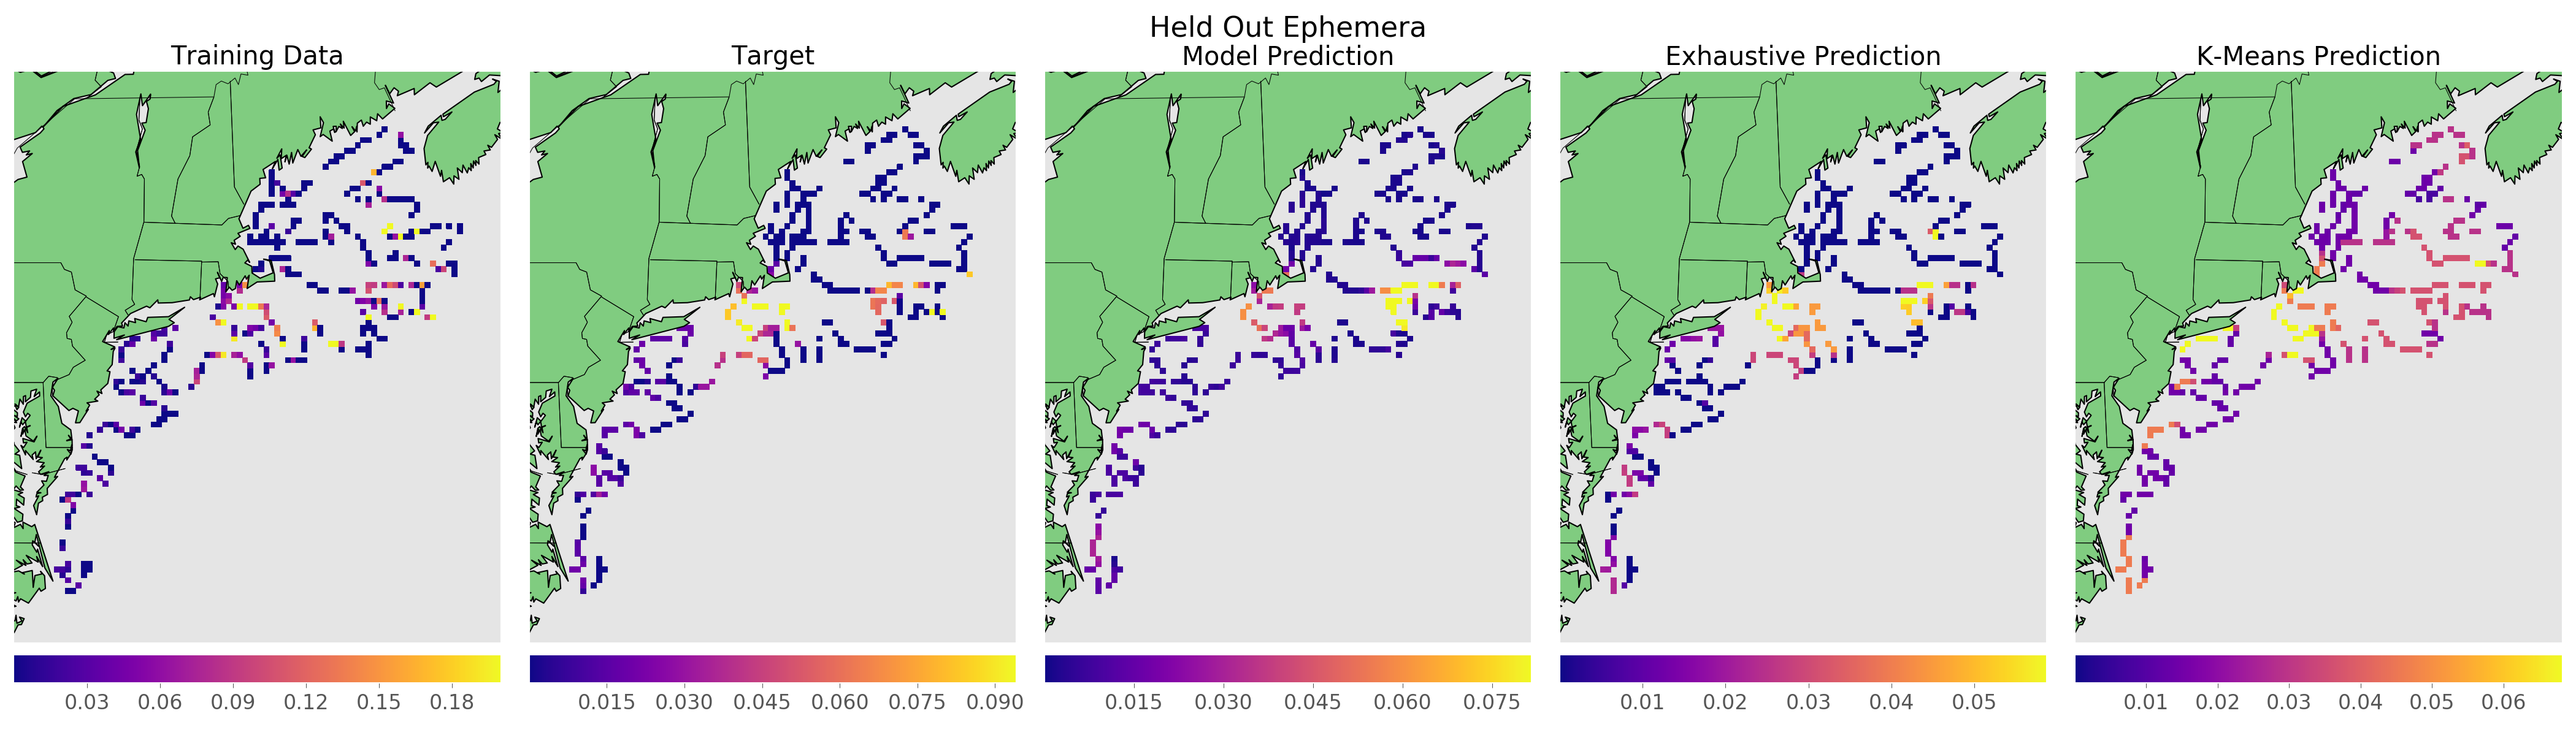
\includegraphics{figures/icra_plankton/maps_Ephemera_8}\\
        %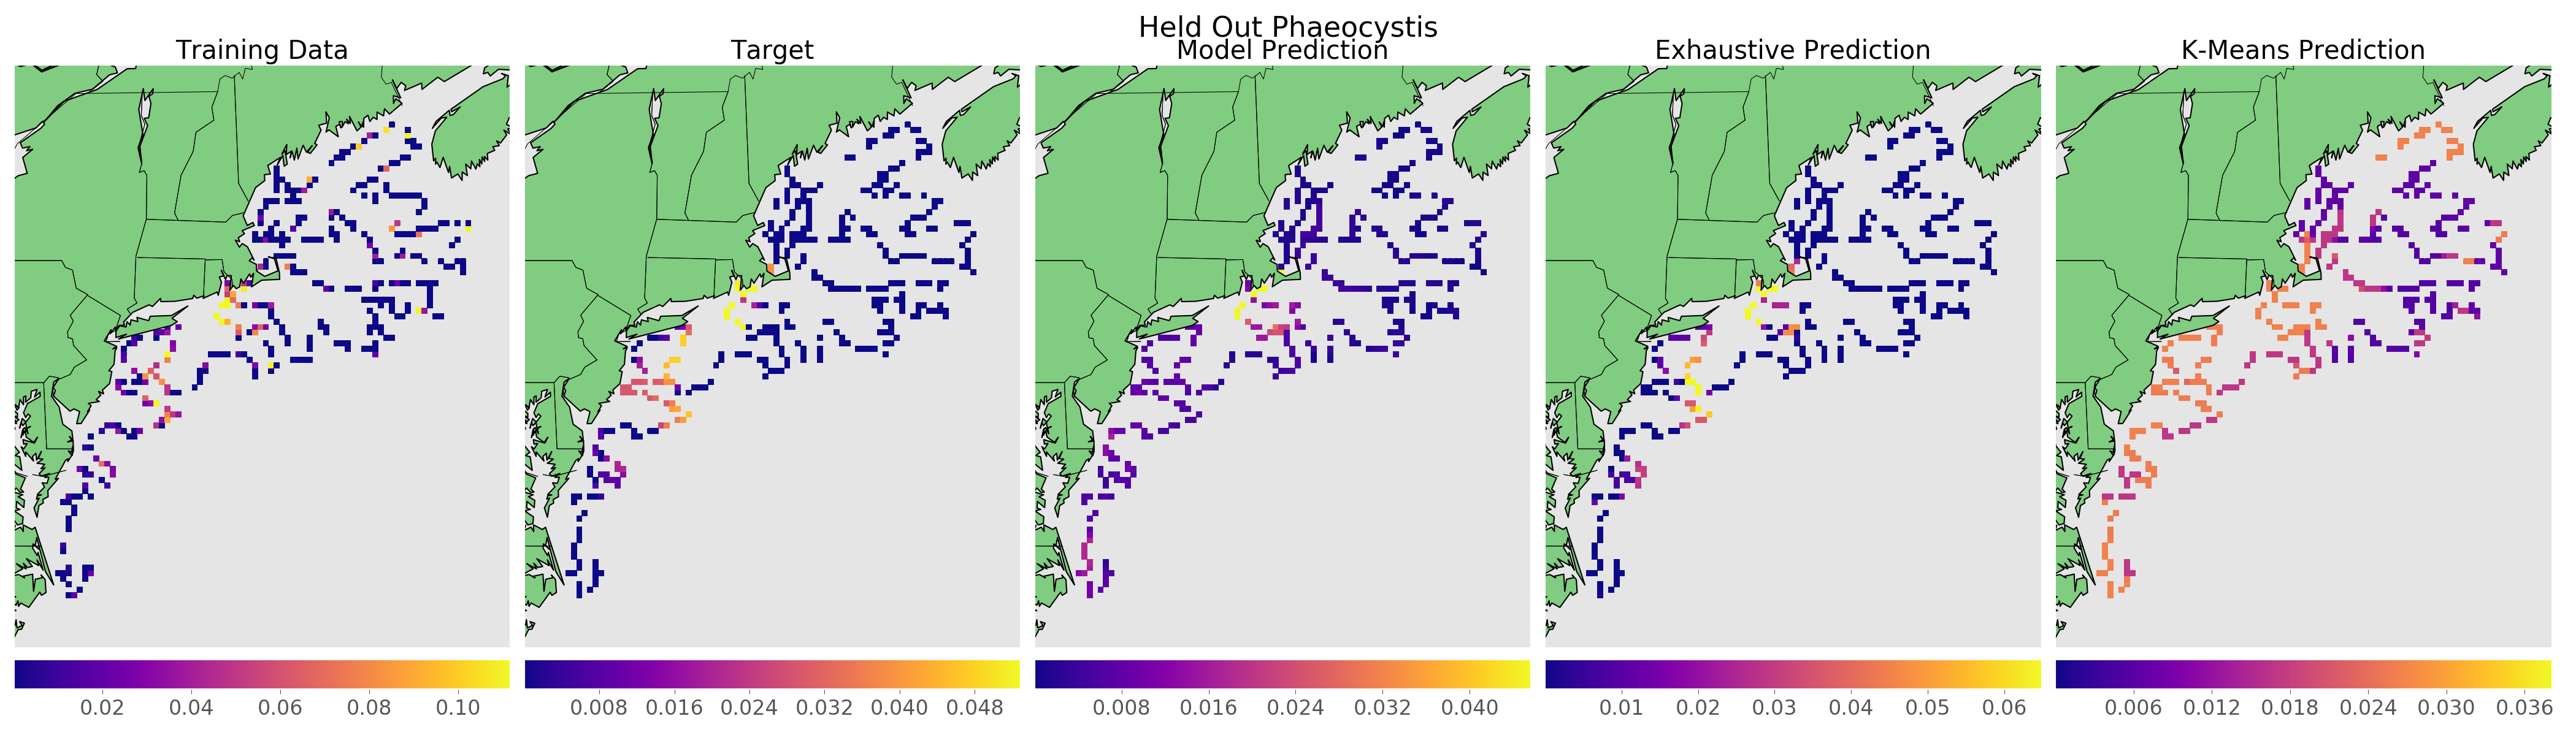
\includegraphics{figures/icra_plankton/maps_Phaeocystis_8}
        \end{tabular}%
    }
    \caption{Spatial distribution for four target classes (rows) in interleaved training/testing samples. The columns correspond to training data (col. 1), held-out target locations (col. 2), and the three models under evaluation (col. 3-5). We find close correspondence between the proposed model and the target data, but exhaustive nearest-neighbor approach has the most similar distribution to held-out target locations. This is because the distribution of plankton is correlated with its spatial neighbors, and hence simple interpolation of the training data is likely to give an accurate plankton distribution at the held-out locations.}
    \label{fig:plankton-pisces-maps-8}
\end{figure}
\begin{figure}
    \centering
    \resizebox{0.9\textwidth}{!}{%
        \begin{tabular}{c}
        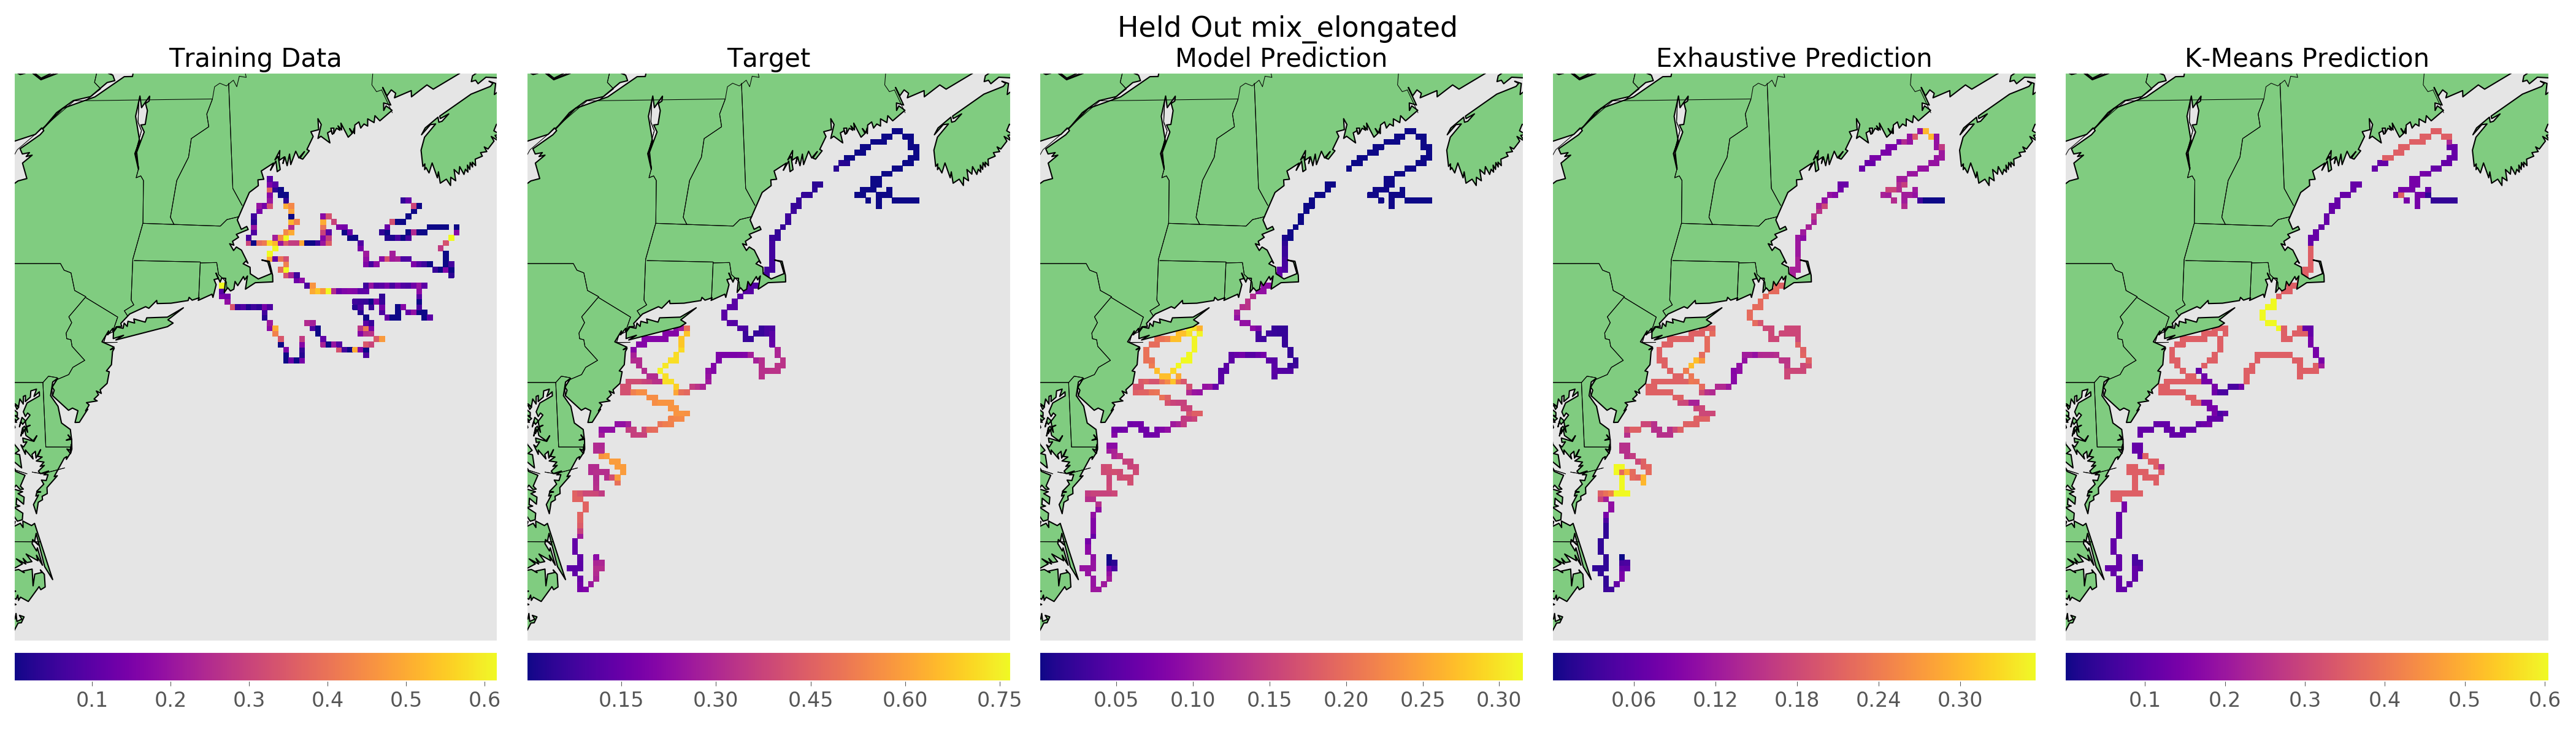
\includegraphics{figures/icra_plankton/maps_mix_elongated_1} \\
        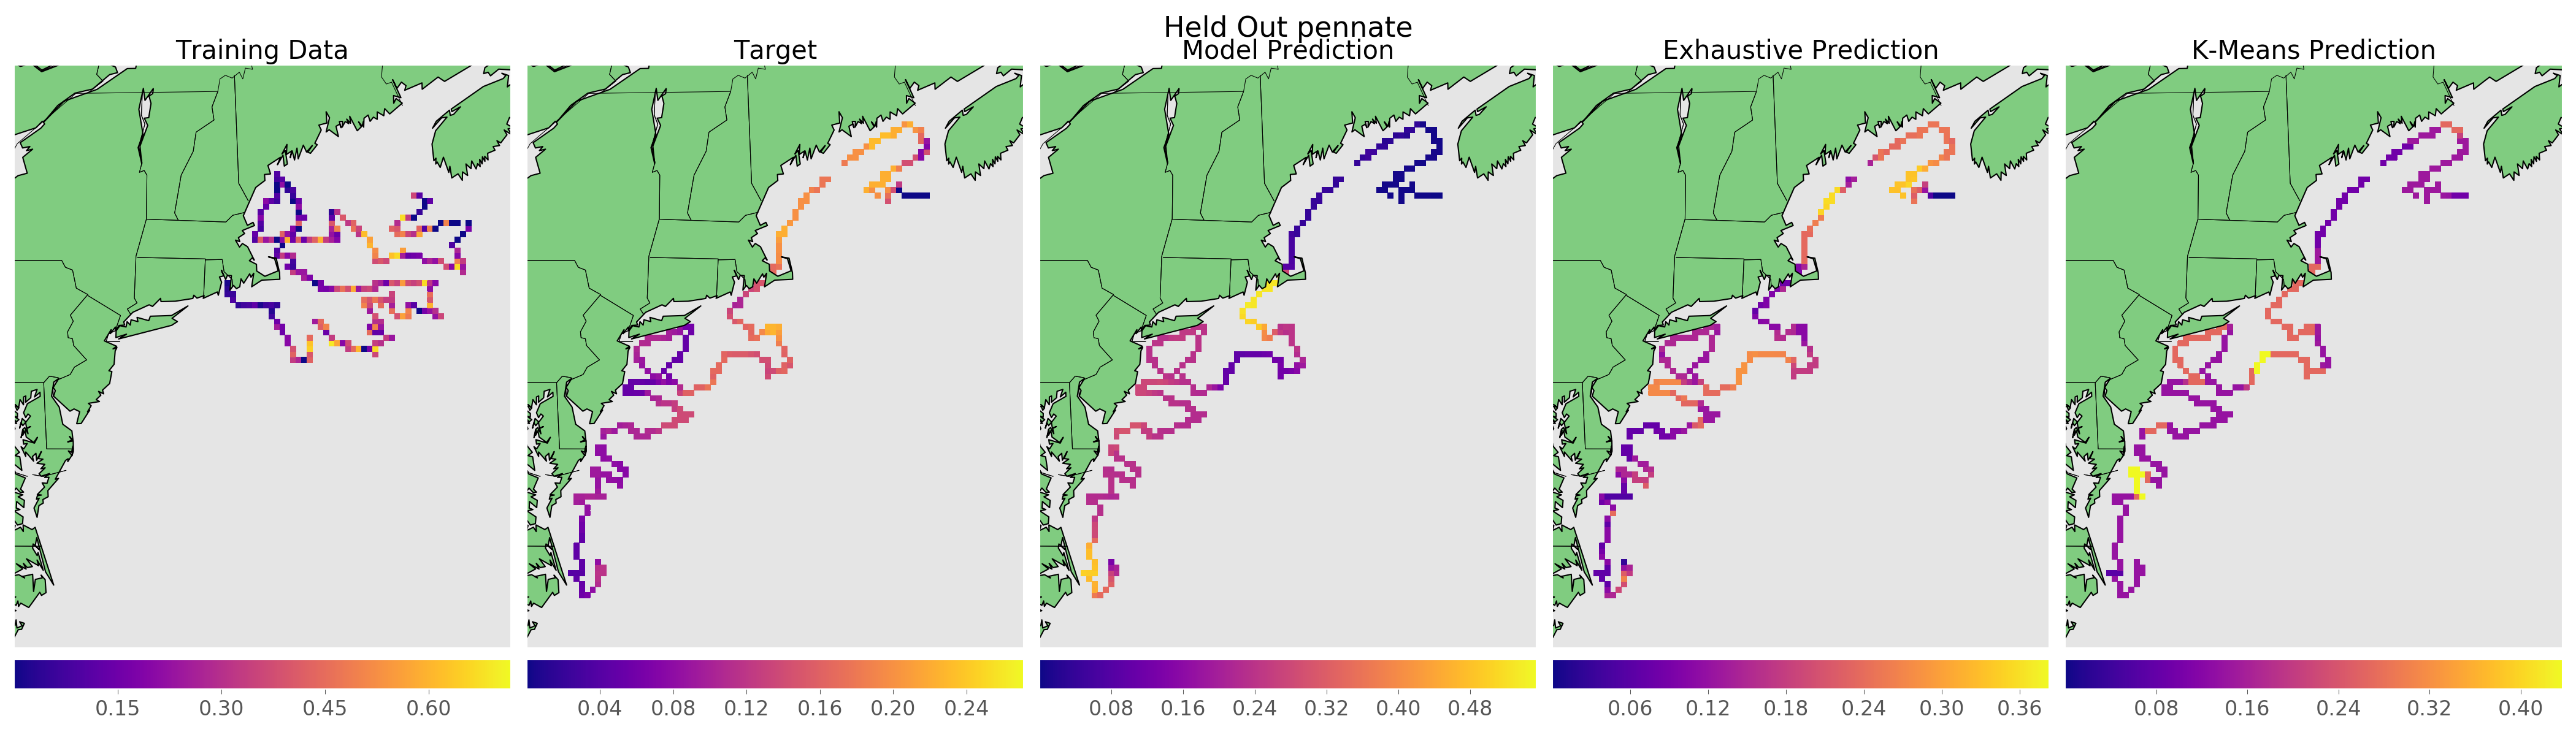
\includegraphics{figures/icra_plankton/maps_pennate_1}\\
        %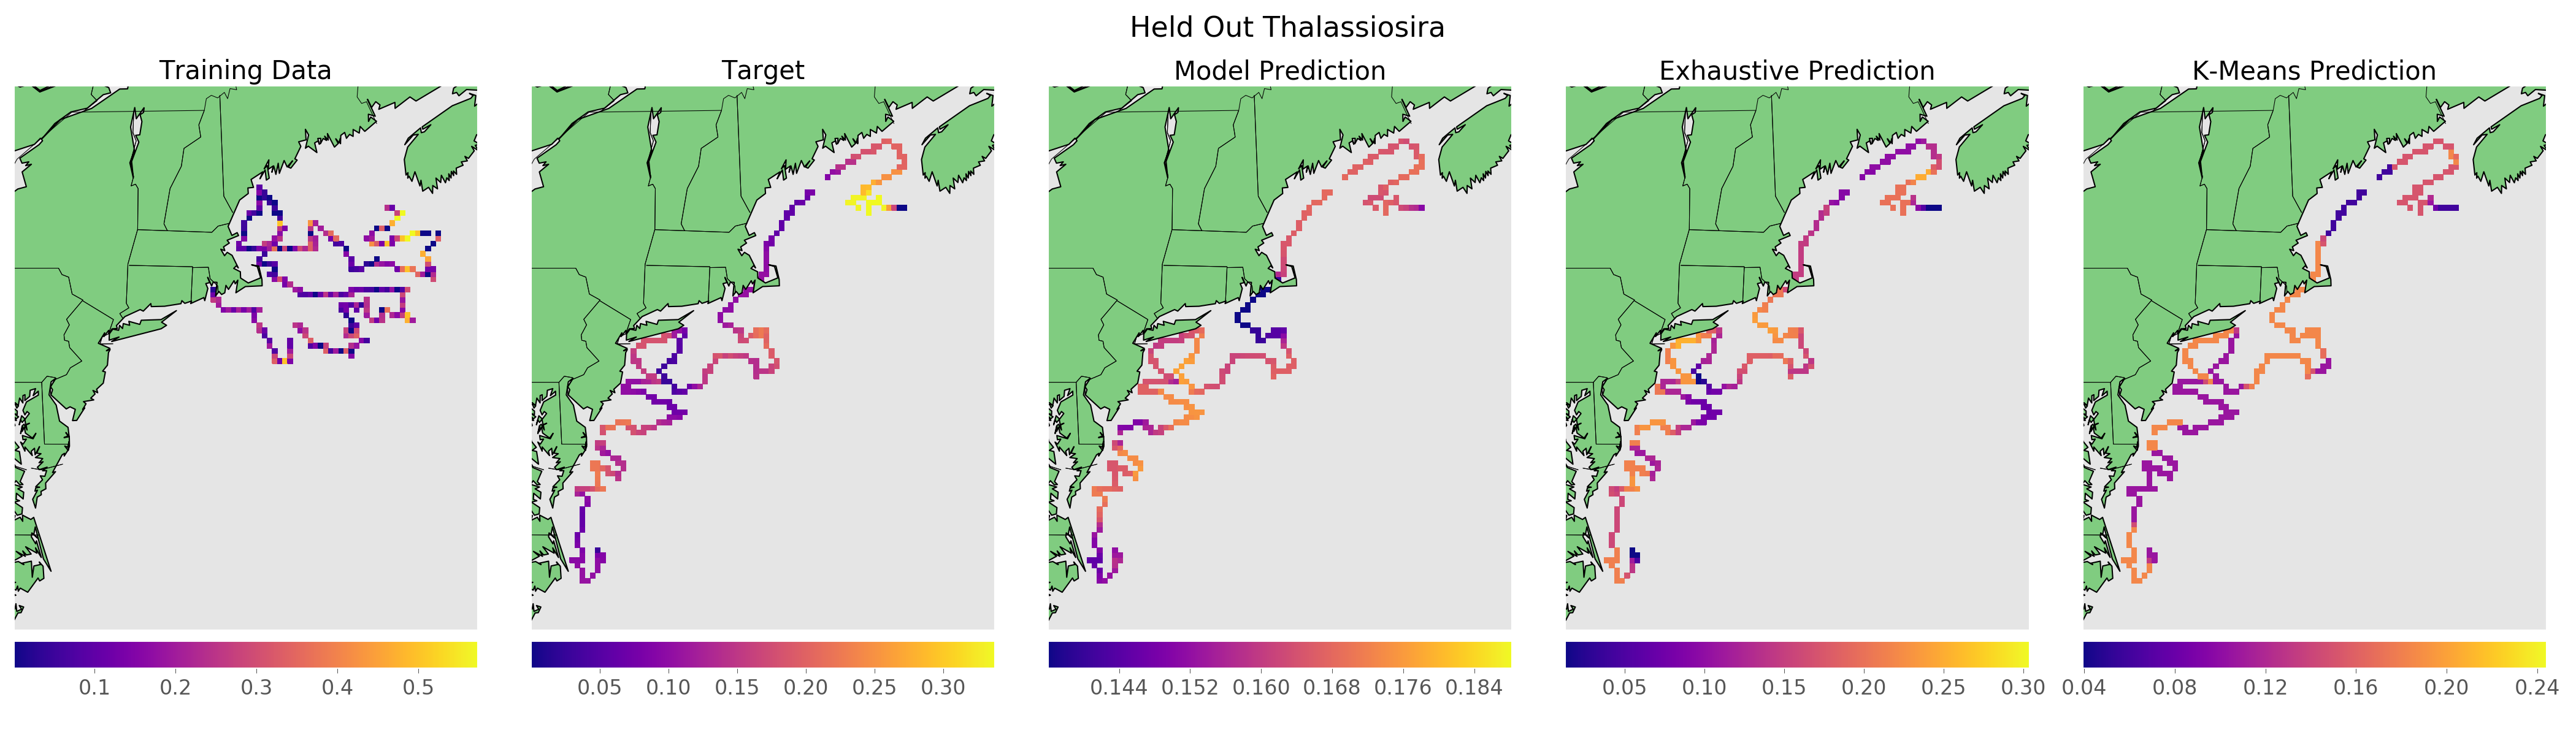
\includegraphics{figures/icra_plankton/maps_Thalassiosira_1}\\
        % 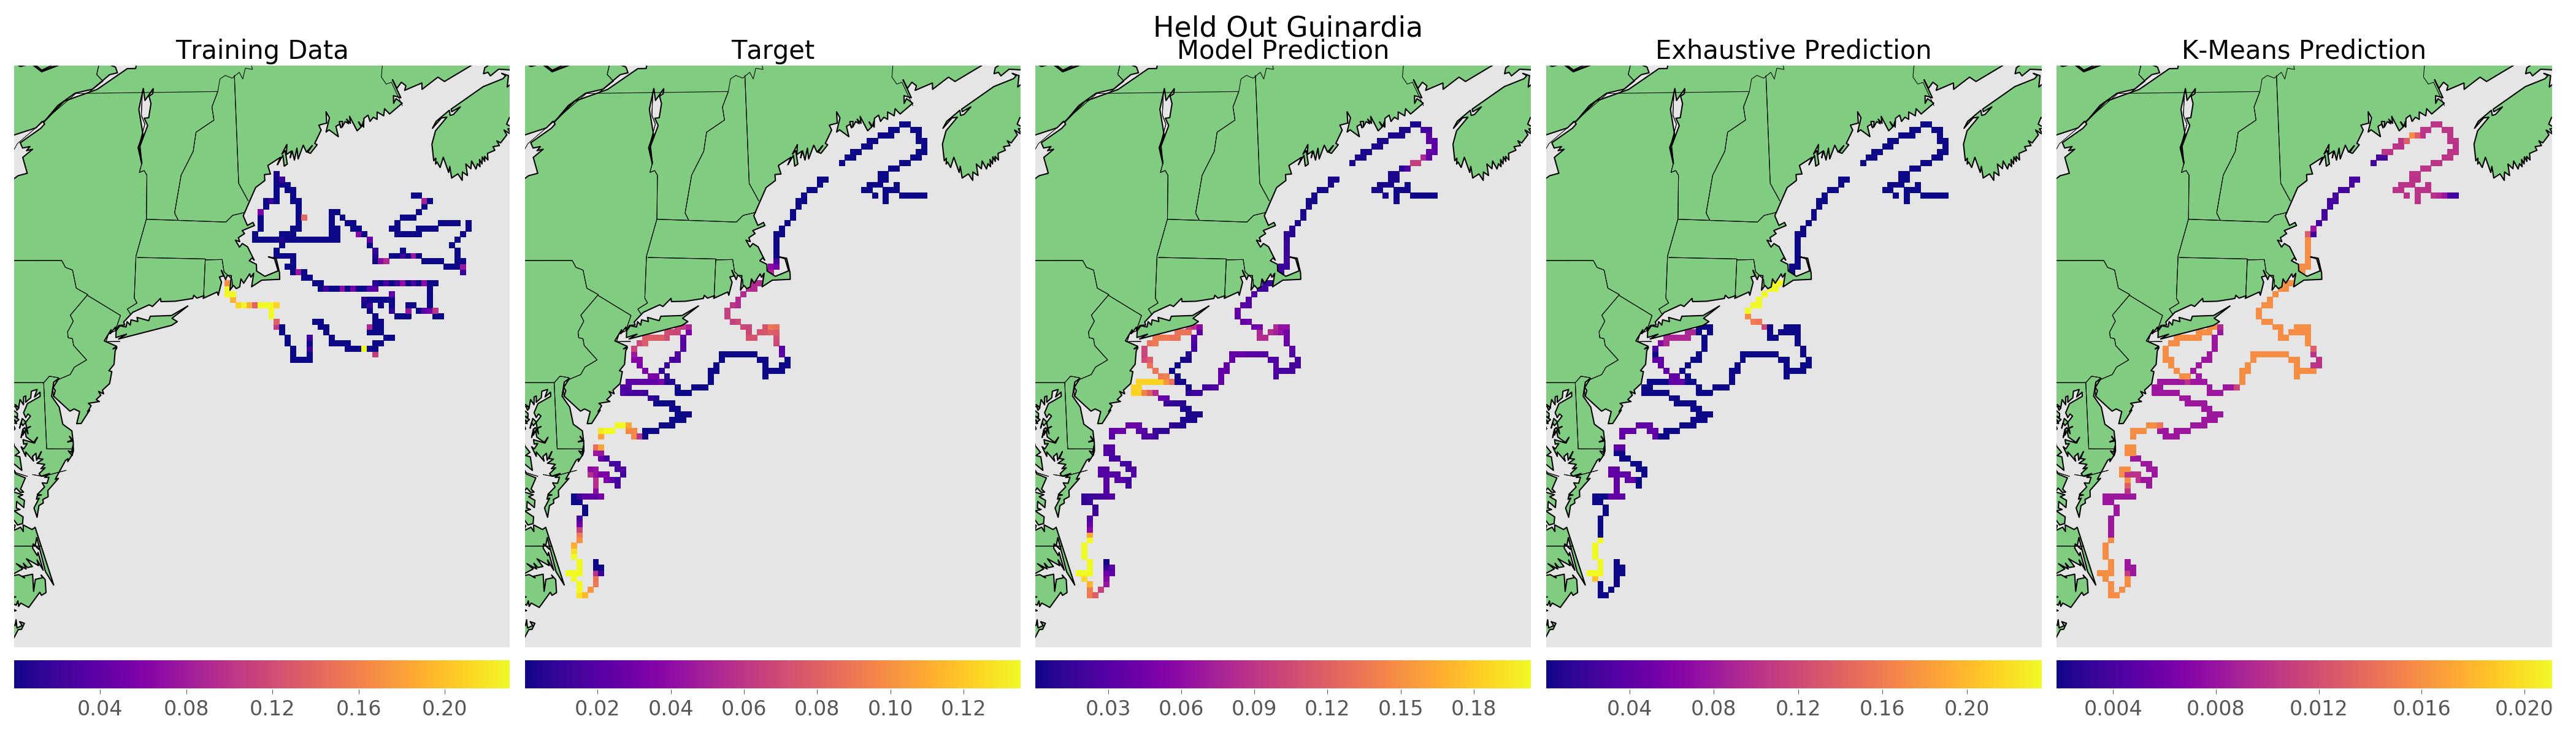
\includegraphics{figures/icra_plankton/maps_Guinardia_1}\\
        % 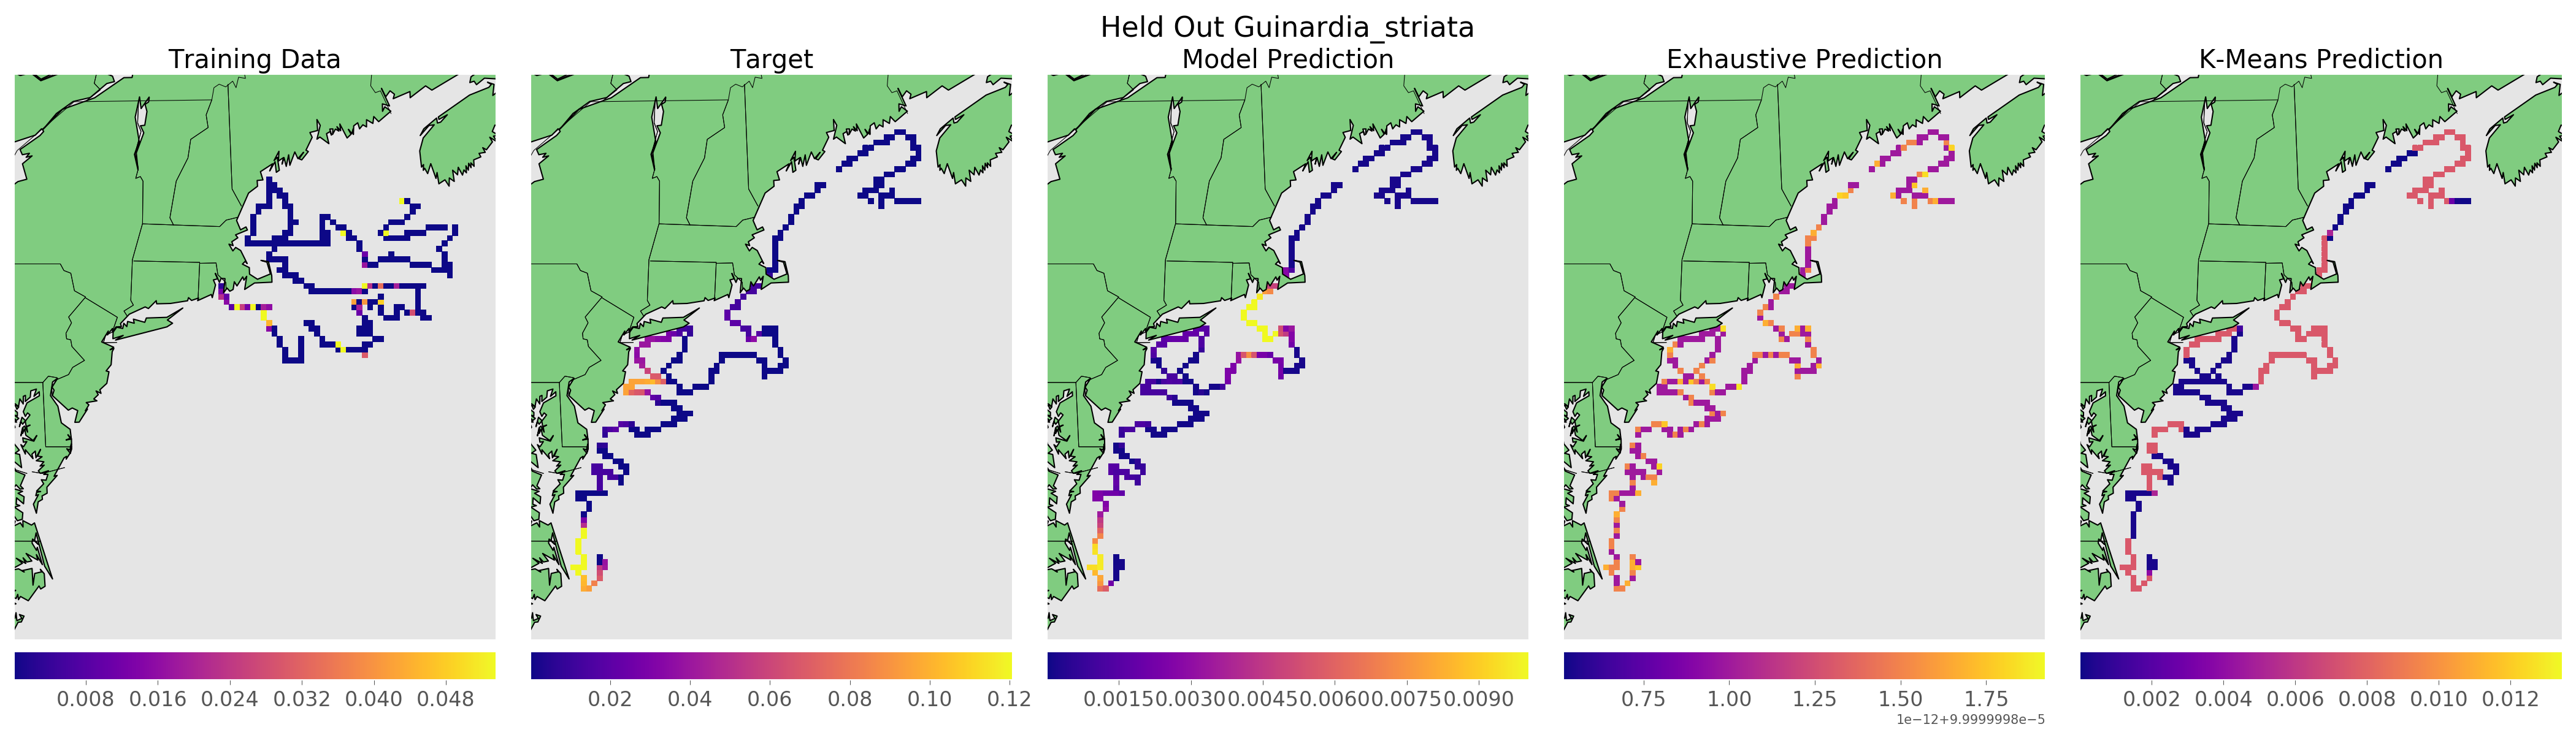
\includegraphics{figures/icra_plankton/maps_Guinardia_striata_1}\\
        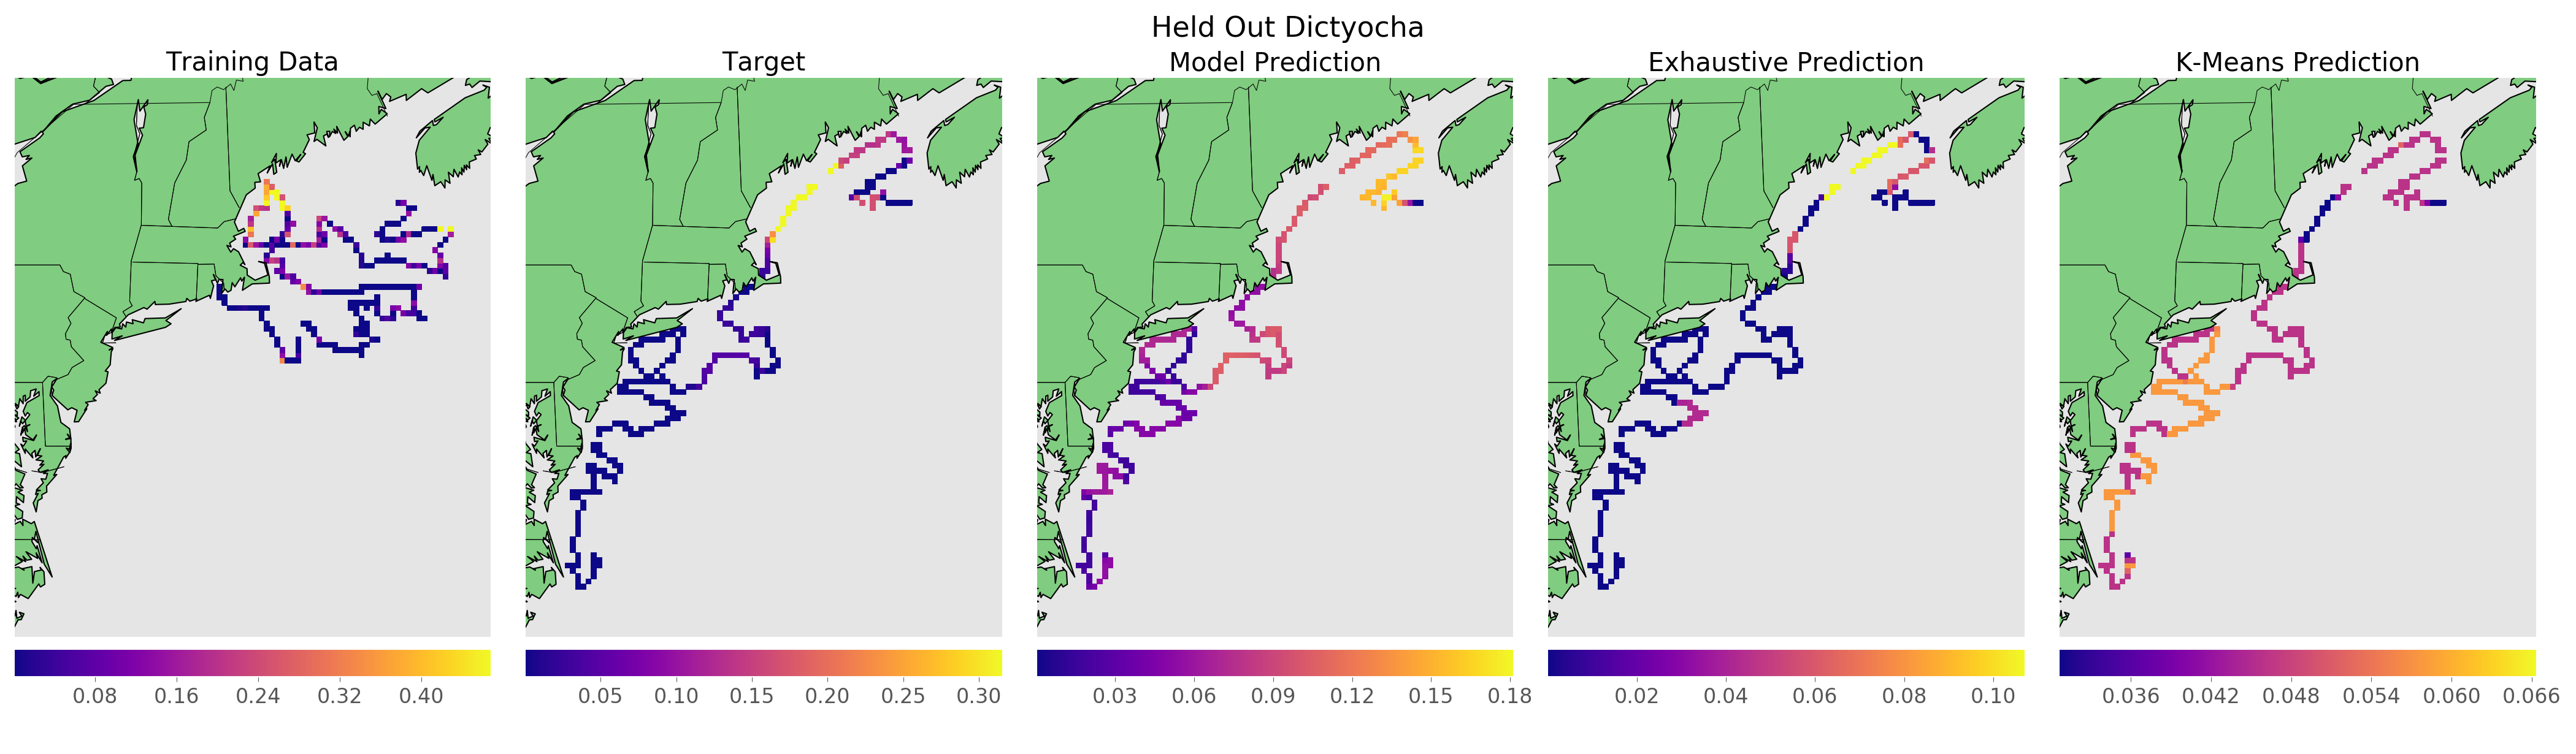
\includegraphics{figures/icra_plankton/maps_Dictyocha_1}\\
        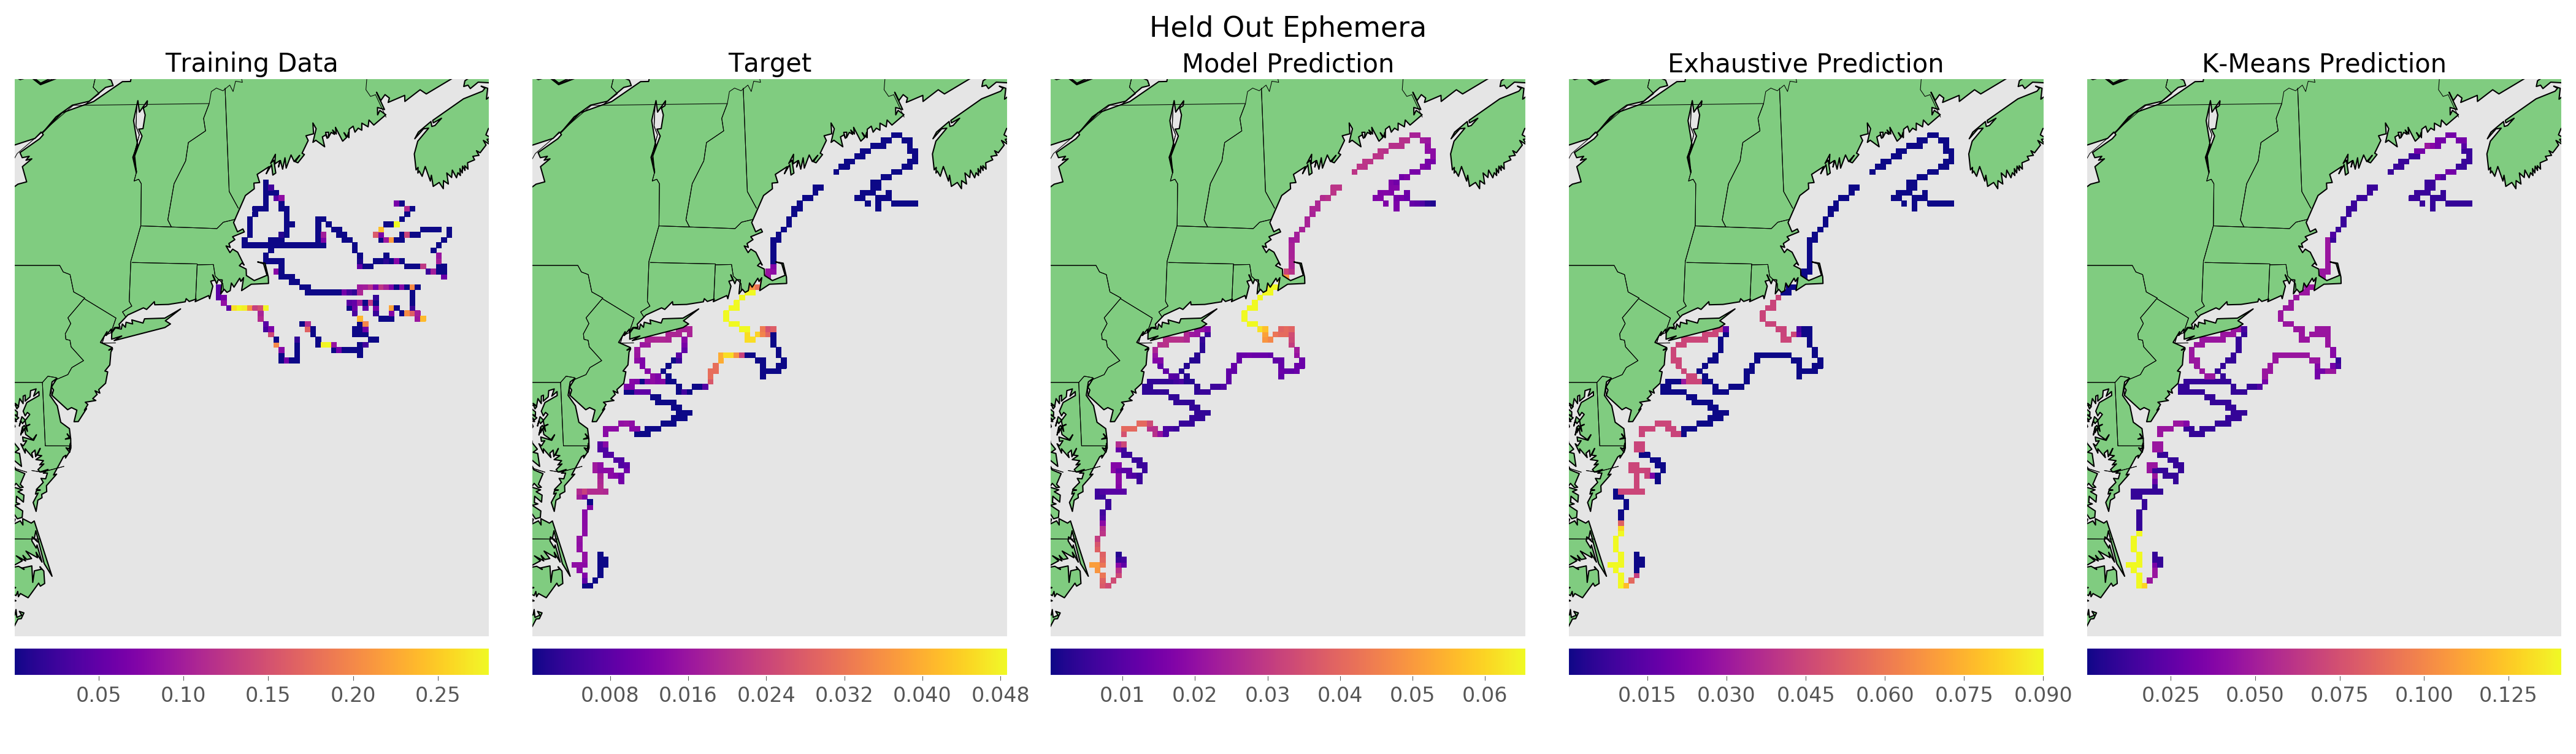
\includegraphics{figures/icra_plankton/maps_Ephemera_1}\\
        %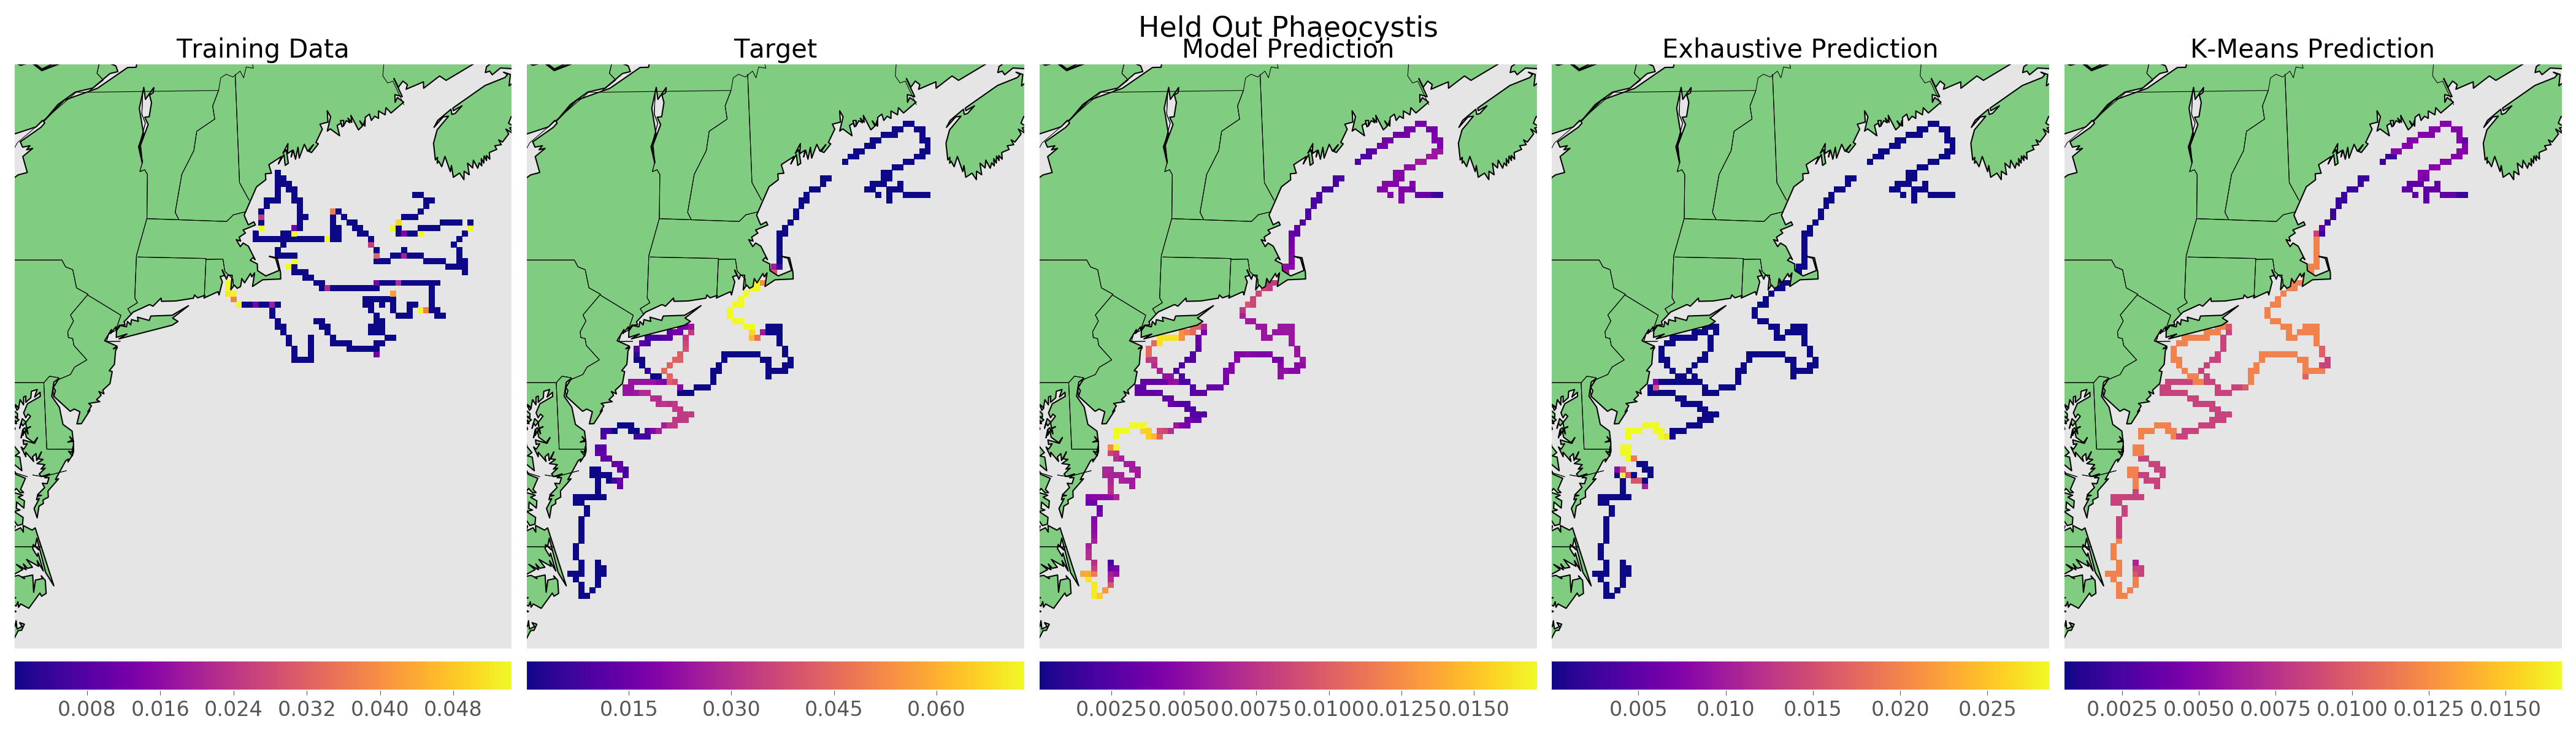
\includegraphics{figures/icra_plankton/maps_Phaeocystis_1}
        \end{tabular}%
    }
    \caption{Spatial distribution for four target classes (rows) in split training/testing samples. The columns correspond to training data (col. 1), held-out target locations (col. 2) , and the three models under evaluation (col. 3-5). The proposed plankton topic model provides predictions that agree better with the held-out observations than do the simpler k-means based plankton community model or the exhaustive nearest neighbor search.}
    \label{fig:plankton-pisces-maps-1}
\end{figure}

We ran our model for a range of choices of the hyperparameters $\alpha, \beta \in$ \{0.001, 0.01, 0.1, 0.5, 1\} and $\gamma \in \{10^{-6},10^{-5},10^{-4}\}$ with each of the top 8 taxa held out of the testing data and for both training regimes. We also ran the exhaustive search and k-means strategies for each. The strategies each produce an estimate for $P(w=v^\star | g(x))$, which we then smooth with a median filter with size parameter $\sigma$. For a scalar threshold $\tau$, we predict that location $x$ is a hotspot if $\Pi_\sigma(P(w=v^\star | g(x))) > \tau$, where $\Pi_\sigma$ is the median function over a square region with side length $\sigma$. 

To evaluate our results we compare the held-out locations in the test set (Fig.~\ref{fig:plankton-pisces-maps-8} and \ref{fig:plankton-pisces-maps-1}, column 2) to predictions from each of the proposed strategies (Fig.~\ref{fig:plankton-pisces-maps-8} and \ref{fig:plankton-pisces-maps-1}, our model, column 3; exhaustive nearest neighbour search, column 4; and k-means search, column 5). The input to the models is illustrated with the observed values of the held-out class at the training locations (Fig.~\ref{fig:plankton-pisces-maps-8} and \ref{fig:plankton-pisces-maps-1}, column 1). Our findings show that the prediction problem is relatively straightforward for the interleaved experiment (Fig.~\ref{fig:plankton-pisces-maps-8}). In contrast, the problem is much more difficult when training and testing locations are in different parts of the world. (Fig.~\ref{fig:plankton-pisces-maps-1}). Despite this, for three (Fig.~\ref{fig:plankton-pisces-maps-8} and \ref{fig:plankton-pisces-maps-1}, rows 1, 2, 4) of the four target classes shown here, the spatial location of maxima of our model's predictions are consistently near the maxima in the target distributions.

Varying $\tau$ for each strategy and parameter setting we can count the true positive, true negative, false positive, and false negative hotspot predictions compared to the top 50 examples in the held-out data. These counts give the precision and recall for each parameter choice, for each $v^\star$. We also accumulate these counts across all $v^\star$ to compute the overall precision and recall for each choice of parameters. We assign each set of parameters a score given by the area under its aggregated precision-recall curve and select the parameter set with the maximum score for further comparisons. For the interleaved experiment, best performance was achieved with $\alpha=0.1, \beta=0.1, \gamma=10^{-5}, \sigma=25 km$ and for the split experiment, $\alpha=0.1, \beta=1.0, \gamma=10^{-5},\sigma=35 km$. We chose the number of centroids for the k-means strategy to be the same as the number of topics in the best performing topic model, $K=9$ for the interleaved experiment, and $K=6$ for the split experiment.

We compare the aggregated and individual class precision-recall curves for the best parameters for each strategy (Fig.~\ref{fig:plankton-pisces-pr}). From the aggregated precision-recall curves, we find that our model significantly outperforms the exhaustive nearest-neighbor and the k-means strategies on the split-samples regime, especially when the required precision is high. This indicates that the top few predictions of our model were more likely to be true hotspots than those of the other strategies. The exhaustive nearest-neighbor strategy barely performs better than random guessing on the split regime, yet it performs extremely well on the interleaved regime. This result is expected as the exhaustive strategy does not reason at all about the underlying association between plankton types. Instead, it depends on having observed a training point whose distribution is similar to every test point. In contrast, our model performs nearly as well on the split regime as the interleaved regime.

Our model also outperforms the k-means strategy on the split-samples regime. Note that the k-means strategy is exactly equivalent to the exhaustive search strategy in the limit where $K$ is the number of training points. Both these strategies rely on a distance measure over the class distributions. The high dimensionality of the distributions acts to the detriment of the divergence measure. As the dimensionality of a space increases, the discriminating power of distance metrics within that space decreases. The amount of data needed to find meaningful clusters grows exponentially with the number of dimensions, a phenomenon sometimes called \textit{the curse of dimensionality}. As a result, the two search-based strategies perform well when test points are very near to training points in taxon distribution space, but when test points are further away, a distance measure is less informative and performance is negatively impacted.

\begin{figure}
	\centering
    \begin{minipage}{\textwidth}
        \subfloat[][]{
            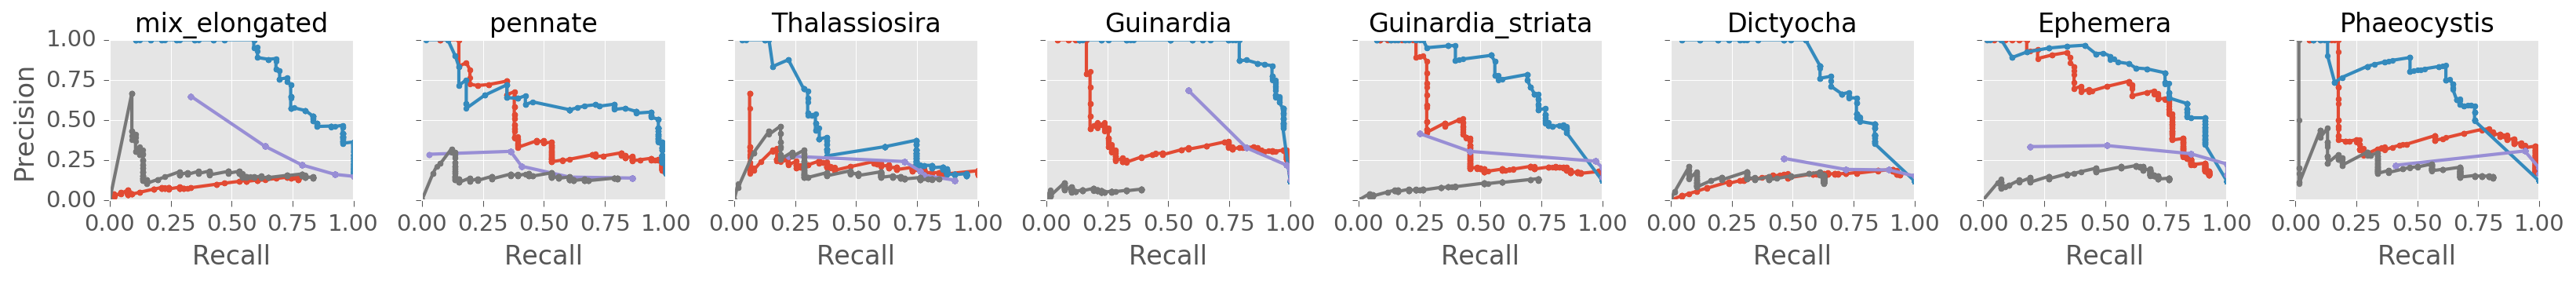
\includegraphics[width=\textwidth]{figures/icra_plankton/pr_8.png}
            \label{fig:plankton-pisces-pr8}
        }\\
       \subfloat[][]{
            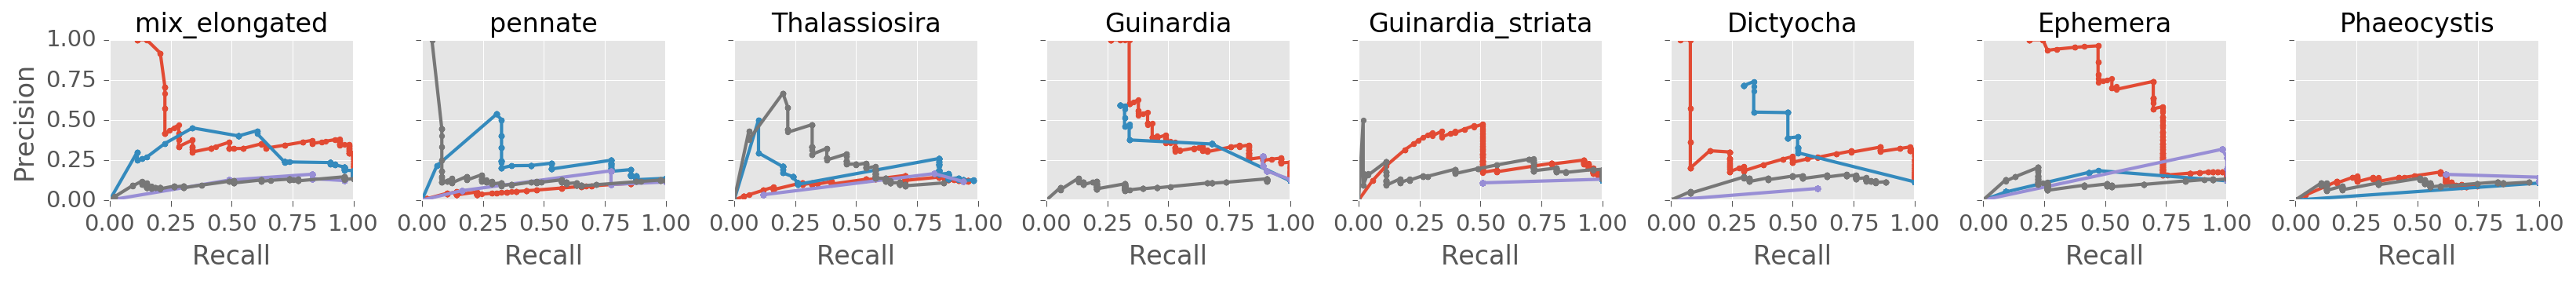
\includegraphics[width=\textwidth]{figures/icra_plankton/pr_1.png}
            \label{fig:plankton-pisces-pr1}
        }
    \end{minipage}\\
    \begin{minipage}{\textwidth}
    	\centering
        \subfloat[][]{
            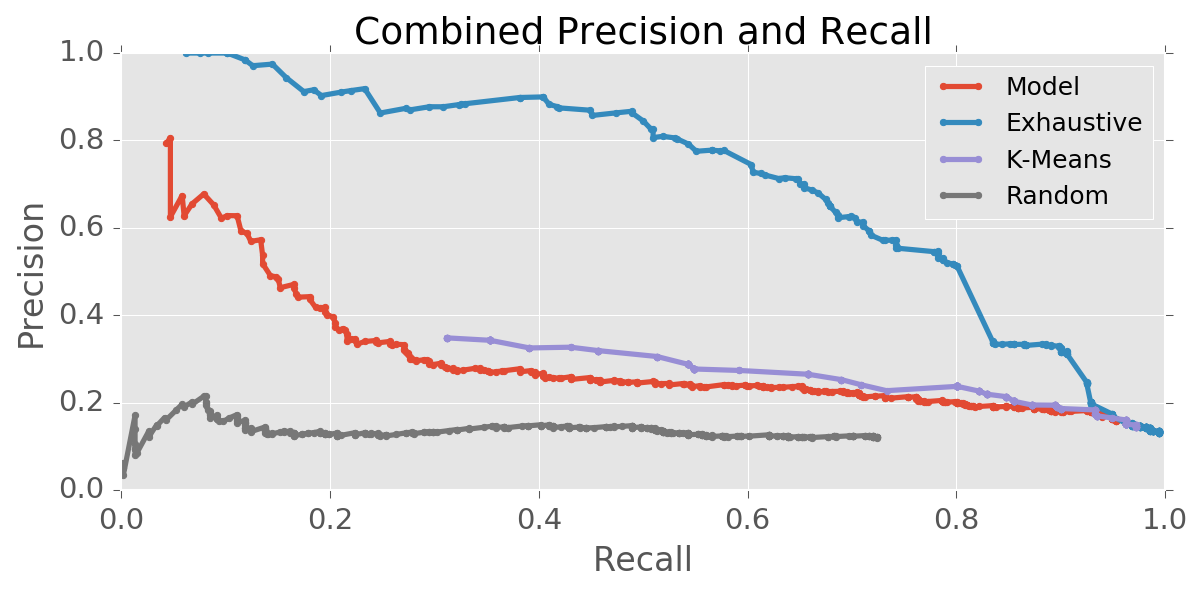
\includegraphics[width=0.48\textwidth]{figures/icra_plankton/pr_summary_8.png}
            \label{fig:plankton-pisces-pr8s}
        }%
        \subfloat[][]{
            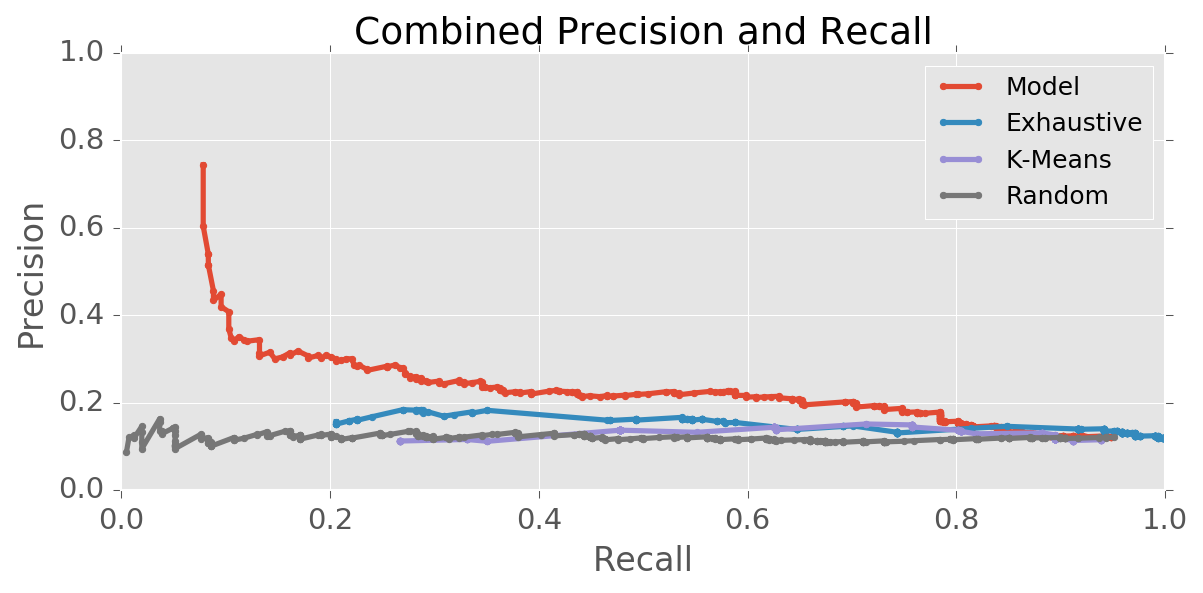
\includegraphics[width=0.48\textwidth]{figures/icra_plankton/pr_summary_1.png}
            \label{fig:plankton-pisces-pr1s}
        }
    \end{minipage}

    \caption
    {Precision vs recall curves for the community model on each of 8 held-out taxa.
	 \protect\subref{fig:plankton-pisces-pr8}, \protect\subref{fig:plankton-pisces-pr8s} Interleaved train and test data.
	 \protect\subref{fig:plankton-pisces-pr1}, \protect\subref{fig:plankton-pisces-pr1s} Split train and test data.
    }
    \label{fig:plankton-pisces-pr}
\end{figure}

\todo[inline]{Need another sentence or two to wrap up the chapter}